\documentclass[12pt, 						% Tamanho da Fonte
			openright, 					% Capítulos tem início em páginas ímpares
			twoside,					% Impressão em anverso e verso
			a4paper,x					% Tamanho do papel A4
			english,					% Idioma adicional para hifenização
			brazil]{abntex2}				% Idioma principal para hifenização

\usepackage[utf8]{inputenc}		% abnTEX usa a codificação UTF8
\usepackage[T1]{fontenc}			% Selecao de codigos de fonte
\usepackage{lmodern}			% Altera a fonte usada para a impressão do documento
\usepackage{relsize}				% Permite a criação de "partes" que contém mais de um capítulo no trabalho

\usepackage{indentfirst} 					% Indenta o primeiro parágrafo de cada seção
\setlength{\parindent}{1.3cm}				% Configura o tamanho do parágrafo
\setlength{\parskip}{0.2cm} 					% Controla o espaçamento entre parágrafos
\OnehalfSpacing						% Espaçamento entre linhas

\setlrmarginsandblock{3cm}{2cm}{*}			% Margens
\setulmarginsandblock{3cm}{2cm}{*}			% Margens
\checkandfixthelayout						% Margens

\usepackage{color}				% Controle das cores
\usepackage{graphicx}			% Inclusão de gráficos
\usepackage{amsmath}			% Expressões Matemáticas
\usepackage{caption}
\usepackage{subcaption}

\titulo{A duração esperada da aposentadoria para \\homens no Brasil: 1980 -- 2025} 			% Título do trabalho
\autor{Matheus Lobo Alves Ferreira}									 			% Nome do autor(a) do trabalho
\data{2015}																% Data do trabalho

%---
% Nome da Instituição
\instituicao{Universidade Federal de Minas Gerais
		\par Instituto de Ciências Exatas
		\par Departamento de Estatística
		\par Programa de Graduação em Ciências Atuariais
 }
%---

\local{Belo Horizonte -- Minas Gerais}									% Localidade de apresentação do trabalho

%---
% Preambulo é o texto impresso na Folha de Rosto e na Folha de Aprovação. Ele deve conter o tipo do documento, o objetivo, o nome da instituição e a área de concentração.

\preambulo{Monografia apresentada ao Departamento de Estatística da Universidade Federal de Minas Gerais como requisito parcial à obtenção do título de Bacharel em Ciências Atuariais.}
%---

\tipotrabalho{Monografia}									% Tipo de trabalho
\orientador{Bernardo Lanza Queiroz}							% Orientador do trabalho

\usepackage{hyperref}  									% Controla a formação do índice
\makeatletter
\hypersetup{
	pdftitle = {\@title},
	pdfauthor = {\@author},
	pdfsubject = {\imprimirpreambulo},
	pdfkeywords = {PALAVRAS}{CHAVE}{EM}{PORTUGUES},
	pdfcreator = {\@author},
	colorlinks = true,
	linkcolor = black,
 	citecolor = black,
	urlcolor = black}
\makeatother

\usepackage{cmap}					% Mapear caracteres especiais no PDF

\usepackage{lastpage}				% Usado para imprimir a ficha catalográfica

\usepackage[brazilian,hyperpageref]{backref}		% Paginas com as citações na bibliografia
\usepackage[alf]{abntex2cite}					% Citações padrão ABNT

% --- 
% Configurações do pacote backref

\renewcommand{\backrefpagesname}{Citado na(s) página(s):~}

% Texto padrão antes do número das páginas

\renewcommand{\backref}{}

% Define os textos da citação

\renewcommand*{\backrefalt}[4]{
	\ifcase #1 %
		Nenhuma citação no texto.%
	\or
		Citado na página #2.%
	\else
		Citado #1 vezes nas páginas #2.%
	\fi}%
% ---

\begin{document}

\imprimircapa							% Imprime capa do trabalho
\imprimirfolhaderosto*						% Imprime a folha de rosto do trabalho

%---
% Dedicatoria

\begin{dedicatoria}
	\vspace*{\fill}
		
	\vspace*{\fill}
\end{dedicatoria}
%---

%---
% Agradecimentos

\begin{agradecimentos}
Ao professor Bernardo Lanza Queiroz, pela orientação, apoio e confiança. 

Aos meus pais e irmão, pelo incentivo e apoio incondicional.

E a todos que fizeram parte da minha formação.
\end{agradecimentos}

%---

%---
% Epigrafe

\begin{epigrafe}
	\vspace*{\fill}
	\begin{flushright}
\textit{“You never really understand a person until you consider things from his point of view... \\ Until you climb inside of his skin and walk around in it.” \\
(Harper Lee, To Kill a Mockingbird)}
	\end{flushright}
\end{epigrafe}
%---

%---
% Resumo em Português

\begin{resumo}
Neste estudo, eu investigo a evolução da taxa de atividade masculina no Brasil durante as últimas três décadas e estimo a duração esperada da aposentadoria dos homens brasileiros. O estudo aponta para uma queda na taxa de atividade masculina, principalmente para os primeiros e últimos grupos etários, causado, principalmente, pelo aumento da escolaridade e programas de proteção social. Em seguida eu uso o modelo Lee--Carter para projetar taxas de mortalidade e de participação e estimo a duração esperada da aposentadoria para o período entre 1980 e 2025. Os resultados indicam que a duração esperada da aposentadoria deve crescer nos próximos anos, saindo de um paratamar de aproximadamente 10\% e chegando a quase 20\% da vida ativa dos homens brasileiros, como consequência da aposentadoria precoce e do aumento da expectativa de vida. Essas tendências indicam uma redução na razão entre  entre contribuintes e beneficiários, afetando assim a premissa básica do equilíbrio financeiro e atuarial dos sistemas estruturados em repartição simples.
\\ \\
\textbf{Palavras-chave:} mortalidade, taxa de atividade, Previdência Social, Lee--Carter, aposentadoria 
\end{resumo}
%---


%---
% Resumo em Inglês

\begin{resumo}[Abstract]
In this paper, I analyze the evolution of male labor force participation in Brazil in the last three decades and estimate the expected length of male retirement. I find a steady decline in the labor force participation of young adults and elderly over time, mostly due to access to education and public pension programs. I also use a stochastic forecast model (Lee-Carter) to forecast mortality rates and labor force participation rates and estimate the expected duration of retirement from 1980 to 2025. My findings indicate that the expected length of retirement might increase in Brazil, from 10\% to 20\% of their working lives, as people leave the labor force at early ages and live longer lives. These trends  reduce the ratio between workers and retirees affecting the basic premise of the PAYGO system. 
\\ \\
\textbf{Key-words:} mortality, labor force participation rate, Lee--Carter, Social Security, retirement
\end{resumo}
%---

%---
% Sumário

\pdfbookmark[0]{\contentsname}{toc}
	\tableofcontents*
\cleardoublepage	
%---	

\textual		% Indica o início dos elementos textuais do trabalho, com isso as páginas passam a ser numeradas
%---
% Introdução

\chapter{Introdução \label{cap1}}
	O envelhecimento da população aumentou a preocupação com a sustentabilidade dos programas de transferência de renda para a população idosa \cite{cutler1990aging, bloom2003demographic, bloom2004global, lee2002fiscal, lee2003intergenerational, lee1994formal}. Se no passado a família servia como principal fonte de recursos para essa parte da população, hoje esses recursos são obtidos de programas criados pelo setor público, e em alguns países, pelo setor privado \cite{costa1998evolution}. De maneira geral, esses programas tem um papel fundamental na redução da taxa de pobreza dos idosos e na redução da diferença de renda entre a população idosa e a população em idade ativa \cite{gruber2001international}. Entretanto, recentemente, a vasta maioria dos programas de transferência de renda tem enfrentado sérios problemas financeiros \cite{bongaarts2004population, bloom}. A maior parte desses programas é baseado no sistema de repartição simples, ou seja, a população economicamente ativa sustenta os benefícios da população idosa, sem nenhum tipo de formação de poupança. O equilíbrio  financeiro e atuarial de tais programas é  muito sensível a eventos demográficos, como o envelhecimento da população, o aumento da razão de dependência, e a redução da idade média de aposentadoria \cite{bongaarts2004population, bloom, turra2011}. \\
	Apesar do grande interesse de pesquisadores em estudar o impacto do envelhecimento populacional em países desenvolvidos \cite{gruber2005social,gruber2008social,wise2004social}, pouco se sabe sobre esse problema em países em desenvolvimento. O Brasil é um caso importante a ser estudado, uma vez que o envelhecimento da população já se apresenta como dos maiores desafios às políticas públicas \cite{turra2005before, turra2011}. Além disso, quando comparado a outros países com nível de desenvolvimento semelhante, o Brasil combina um sistema de seguridade social amplo, com um rápido processo de envelhecimento populacional e a queda na taxa de atividade \cite{turra2011}. De acordo com estimativas da ONU, a razão de dependência idosa, definida como a razão entre a população de 65 anos e mais, e a população em idade ativa será de aproximadamente 36\% em 2050, enquanto a razão observada em 2010 foi de 10\%. \\
	Ao mesmo tempo em que ocorrem mudanças no perfil etário da população, a curva de taxas de atividade masculina apresenta uma tendência de queda, principalmente nos primeiros e últimos grupos etários. \citeonline{chahad2013mercado} justificam a queda observada para os primeiros grupos etários com a redução do trabalho infantil e pelo aumento da escolarização desse grupo, \citeonline{camarano1999vive} afirmam que a queda da taxa de atividade dos idosos é um reflexo do aumento da cobertura do Regime Geral de Previdência Social.\\
	Em 2005, os gastos previdenciários correspondiam a aproximadamente 14\% do PIB e a expectativa é de crescimento para os próximos anos \cite{brasil2003gasto, giambiagi1997despesa, queiroz_figoli}. O Banco Mundial estima que a dívida implícita do regime geral de previdência social brasileiro é 3,5 vezes o PIB, a maior considerando países em desenvolvimento \cite{holzmann2004implicit}. \\
	É nesse contexto de aumento da expectativa de vida e queda na taxa de atividade masculina que esse estudo está estruturado. Usando o modelo Lee--Carter e os dados da \textit{Latin America Human Mortality Database} e da PNAD para projetar taxas de mortalidade e de atividade, busca-se obter estimativas confiáveis para estimar a duração esperada da aposentadoria de homens brasileiros (ELRP). Essa medida leva em conta os ganhos da expectativa de vida ocorrida nas últimas décadas e a queda das taxas taxas de atividade observada em anos recentes \cite{queiroz2007determinants}, diferente do que é feito atualmente pelo Ministério da Previdência Social, que assume constante o nível de atividade dos contribuintes do Regime Geral de Previdência Social \cite{projeccao}. \\
	Nesse estudo, aposentadoria é definida como a saída permanente do mercado de trabalho, e, de acordo com \citeonline{lee2001expected} a saída permanente do mercado de trabalho começa a ocorrer por volta dos 50 anos de idade. \\
	Os resultados apontam para o aumento da duração esperada da aposentadoria, sempre acompanhado do aumento da expectativa de vida, além disso, os resultados são consistentes com aqueles encontrados por \citeonline{lee2001expected}, o que fortalece o estudo. A ELRP permite estimar a duração dos compromissos atuariais do Regime Geral de Previdência Social com seus beneficiários, sendo uma ferramenta importante para o planejamento orçamentário do regime.
%---

%---
% Revisão de Literatura

\chapter{Contextualização \label{cap2}}
	\section{A previdência social no Brasil \label{sec1.1}}
	O sistema previdenciário no Brasil é composto por quatro segmentos, o Regime Geral de Previdência Social, os Regimes Próprios de Previdência Social, as Entidades Fechadas de Previdência Complementar e as Entidades Abertas de Previdência Complementar. Devido ao elevado gasto do Regime Geral, cerca de14\% do PIB em 2005 \cite{queiroz_figoli}, esse estudo tem como alvo os seus participantes e beneficiários, entretanto, estudos semelhantes podem ser conduzidos para os demais segmentos. \\
	De acordo com \citeonline{alem1998aposentadoria} a Lei Eloy Chaves (decreto-lei 3.827, de 15 de janeiro de 1923) pode ser considerada, efetivamente, o ponto de partida do sistema previdenciário brasileiro. Essa lei determinava a criação de caixas de aposentadorias e pensões nas empresas ferroviárias existentes na época. Cada empresa possuía uma caixa destinada a amparar seus empregados na inatividade. A administração das caixas eram feitas por um colegiado, composto, em partes iguais, por representantes dos empregados e dos empregadores, sem a participação do Estado. Os autores também afirmam que no decorrer das décadas de 20 e 30 o sistema foi estendido a empresas de diversas categorias profissionais.\\
	\citeonline{oliveira1997reforma} destacam que com a criação do Ministério do Trabalho, Indústria e Comércio na década de 30, a previdência social passou a merecer maior atenção por parte do Estado. A partir desse momento, a vinculação passou a ser feita pela categoria profissional, e não mais pela empresa. Foram criados os institutos de de aposentadorias e pensões e a cobertura previdenciária foi estendida à maior parte dos trabalhadores urbanos. \\
	Embora os institutos proporcionassem cobertura a uma grande parcela dos trabalhadores urbanos, as disparidades entre os planos de benefícios oferecidos por cada um deles permaneceram principalmente pelas diferenças na capacidade financeira de cada instituição \cite{oliveira1997reforma}. Como a contribuição era feita tendo como base o salário dos empregados, os institutos que representavam categorias de profissionais mais abonadas obtinham maiores recursos. \\
	A centralização do sistema previdenciário não ocorreu até a aprovação da Lei Orgânica da Previdência Social em 1966 \cite{oliveira1989previdencia}. O instituto Nacional da Previdência Social (INPS) passou a administrar todos os recursos dos institutos de aposentadorias então existentes \cite{turra2005before}. Outra mudança significativa foi a mudança do regime de capitalização para o regime de repartição simples \cite{leite1983seculo}. \\
	A constituição de 1988 trouxe uma grande reforma previdenciária, ampliando a cobertura do sistema, que passou a  incluir grupos anteriormente excluídos, como os trabalhadores rurais, sem requerer o pagamento de contribuições. Outras medidas também fizeram com que o sistema se tornasse mais generoso, como o estabelecimento do benefício mínimo igual ao salário mínimo e a redução da idade mínima para aposentadoria \cite{stephanes1998reforma}. \\
	Até 1998, benefícios integrais eram concedidos a todos os trabalhadores com 10 anos de contribuição, e que tivessem atingido a idade mínima para aposentadoria (65 anos para homens e 60 para mulheres). Adicionalmente, pessoas que comprovassem um determinado número de anos de trabalho (35 para homens e 30 para mulheres) tinham direito ao recebimento de benefícios previdenciários mesmo sem o pagamento de contribuições ao regime. \\
	Em 1998, com a introdução do fator previdenciário, uma medida atuarial passou a ajustar o valor dos benefícios concedidos tendo como base a expectativa de vida na idade de concessão do benefício, o histórico salarial do participante, e um fator cujo objetivo é desestimular a aposentadoria precoce \cite{queiroz_figoli}. \\
	Em 2015 foi aprovada a Lei Nº 13.183, que determina novas regras para a concessão da aposentadoria por tempo de contribuição por meio da fórmula 85/95 Progressiva. O cálculo levará em consideração o número de pontos alcançados somando a idade e o tempo de contribuição do segurado. Alcançados os pontos necessários, será possível receber o benefício integral, sem aplicar o fator previdenciário.
	\section{A dinâmica demográfica brasileira \label{sec1.2}}
	A transição demográfica é um processo de mudança no perfil etário da população, decorrente da  queda das taxas de mortalidade e fecundidade \cite{brito2008transiccao}. O processo se manifesta, no longo prazo, através do aumento da expectativa de vida e do crescimento da população mais idosa, consequência da queda das taxas de mortalidade e da queda das taxas fecundidade, respectivamente. A figura~\ref{fig0} apresenta a estrutura etária da população brasileira na década de 70 e a estrutura projetada para o ano de 2050.\\
	\begin{figure}[!htb]
	\caption{\label{fig0} Pirâmide Etária: Anos Selecionados}
		\begin{subfigure}[b]{0.5\textwidth}
		\begin{center}
			\caption{\label{fig0.1} Brasil 1970}
			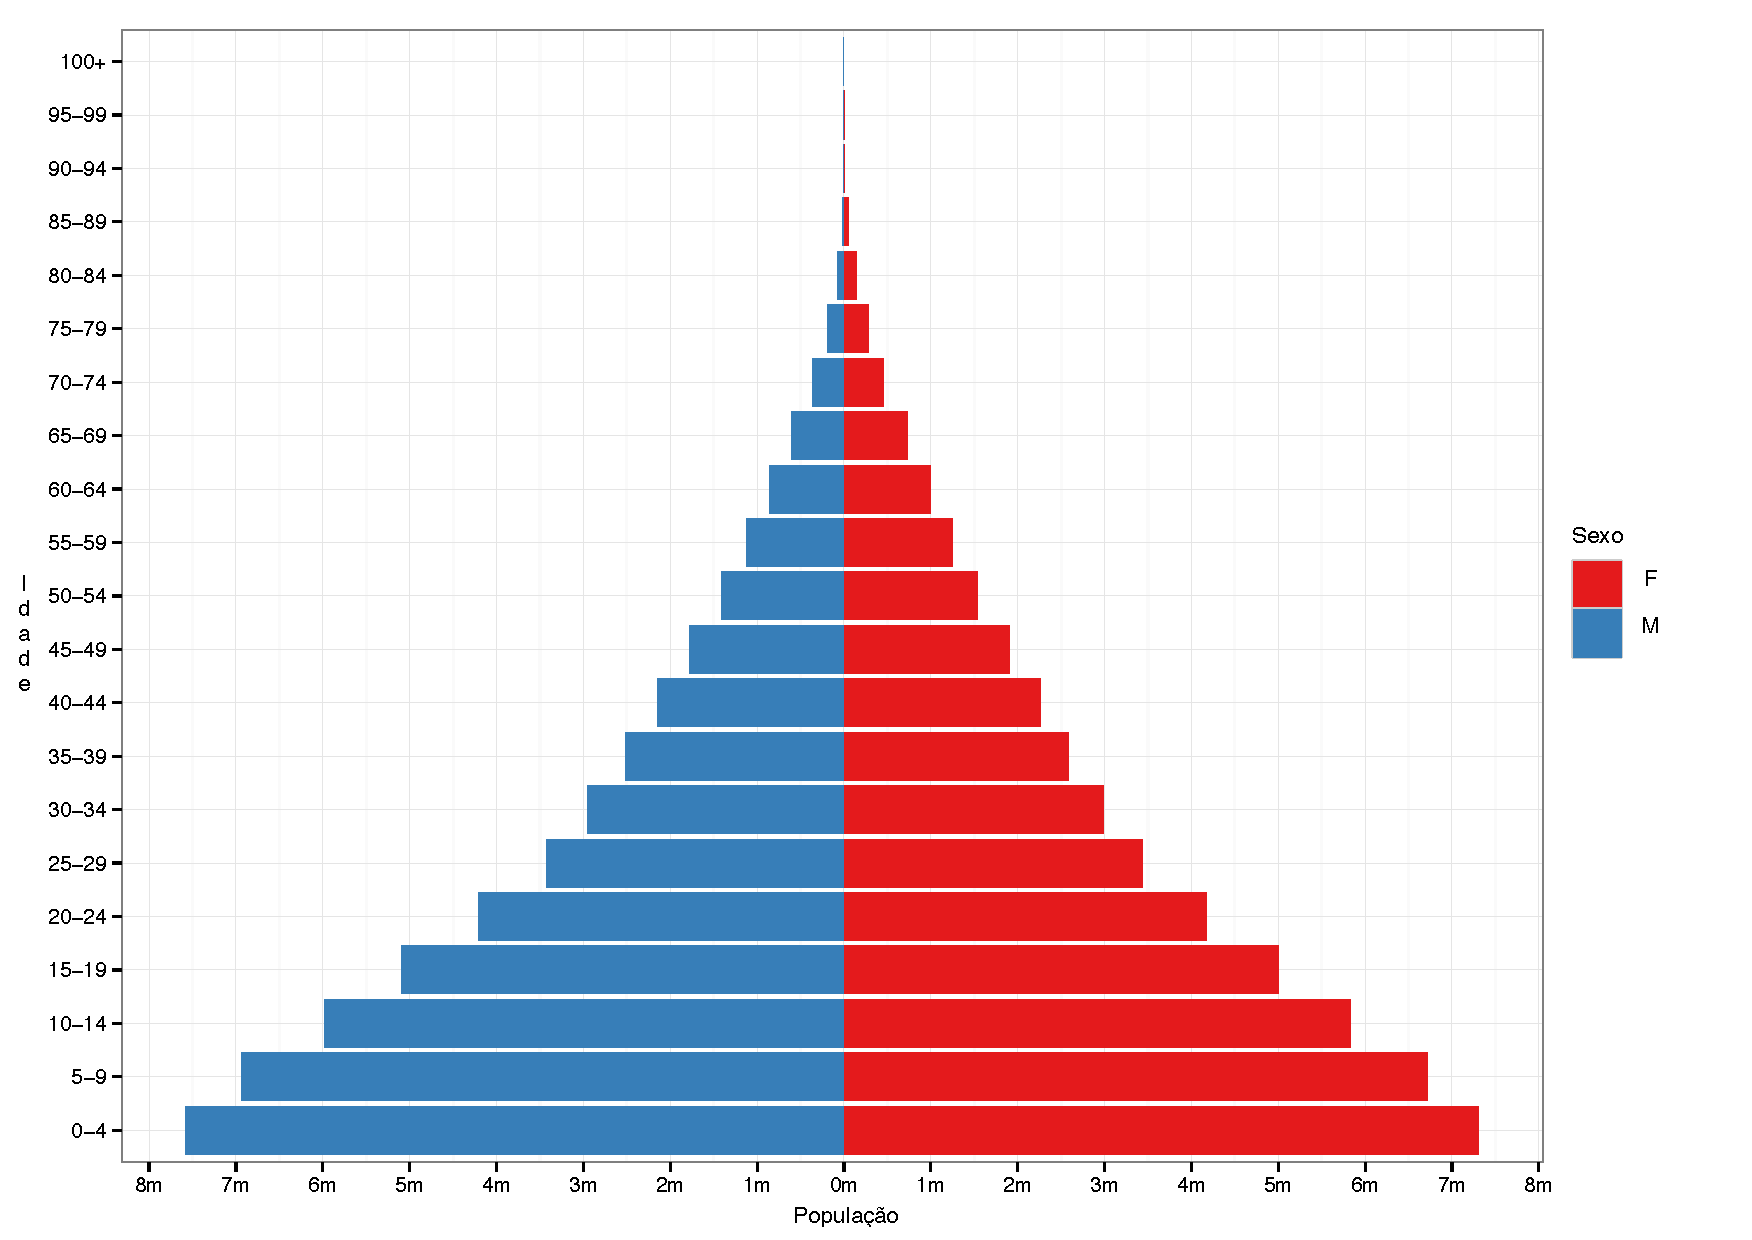
\includegraphics[width=\textwidth]{Graphs/1970.pdf}
		\end{center}
		\end{subfigure}
	\hfill
		\begin{subfigure}[b]{0.5\textwidth}
		\begin{center}
			\caption{\label{fig0.2} Brasil 2050}
			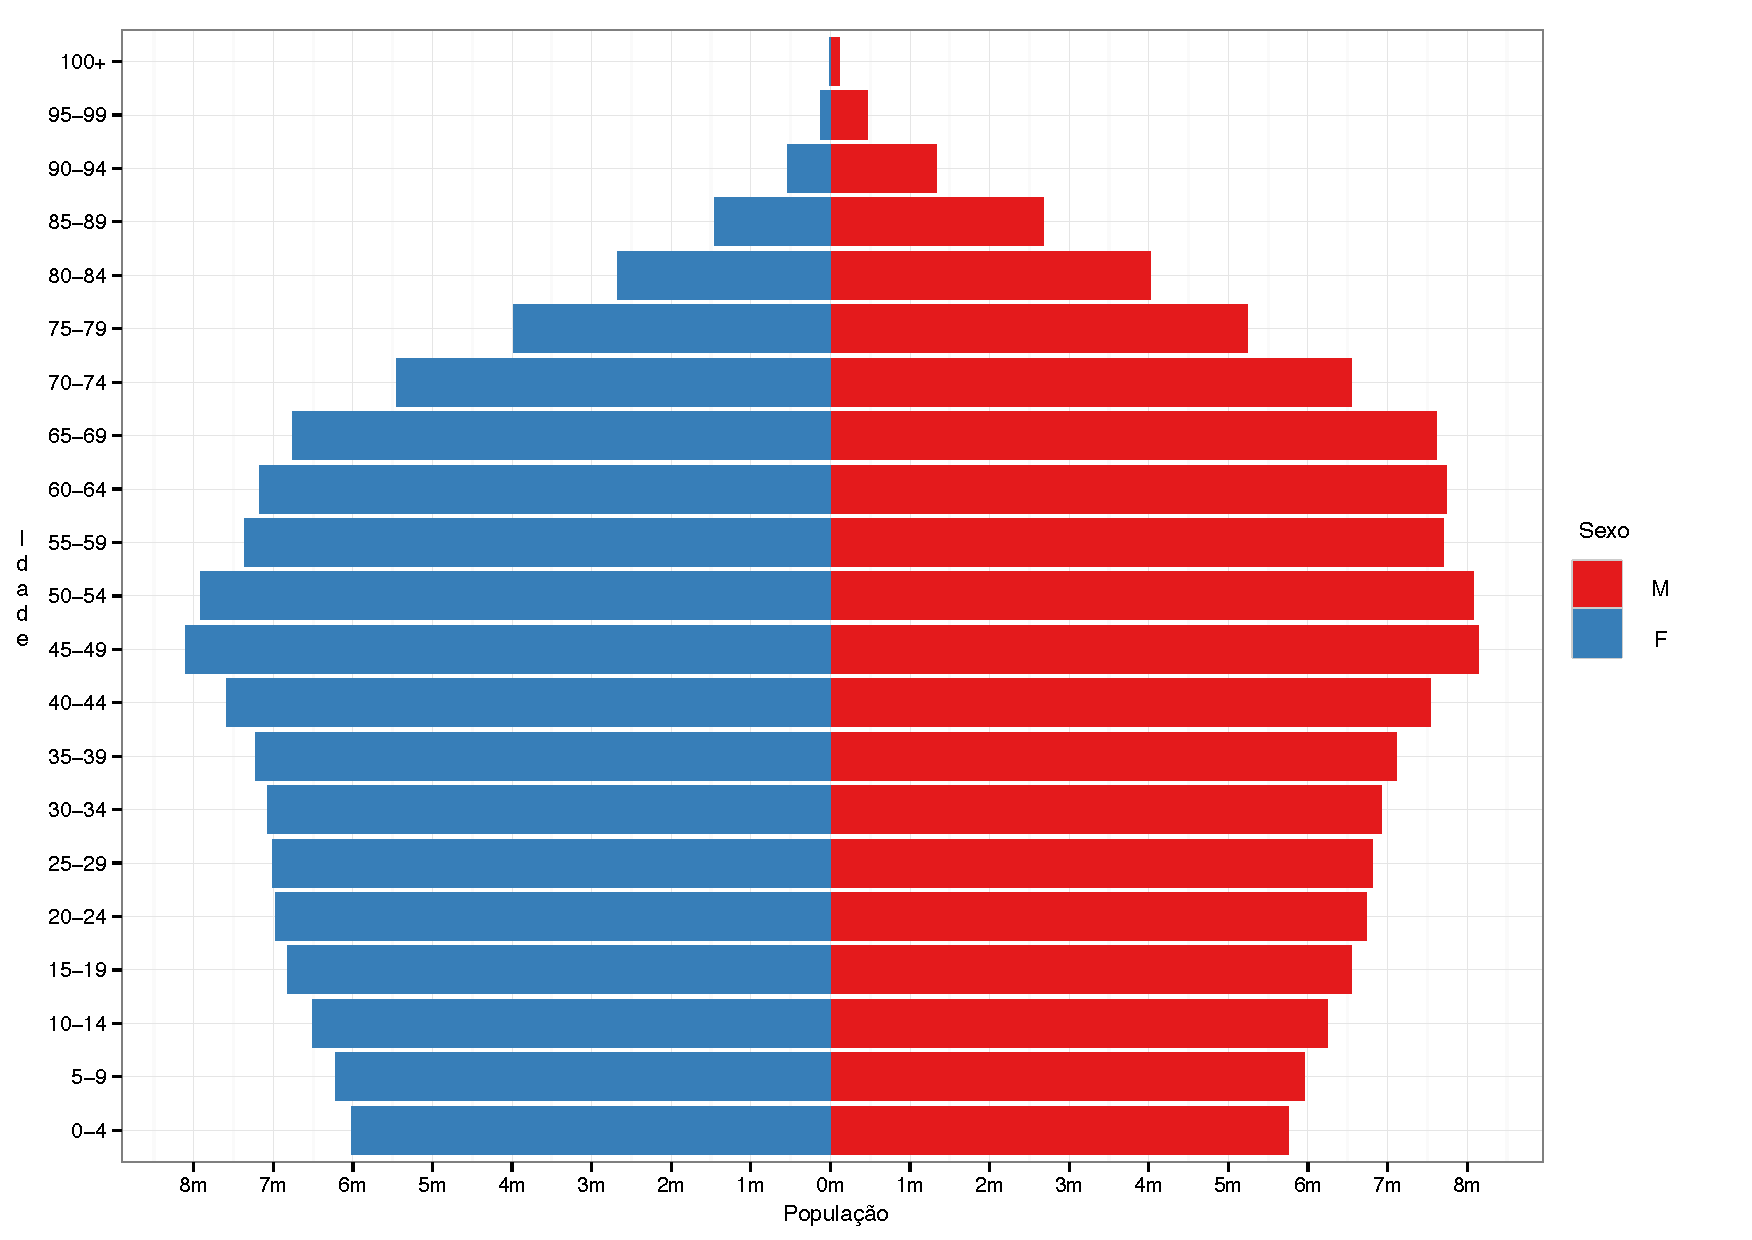
\includegraphics[width=\textwidth]{Graphs/2050.pdf}
		\end{center}
 		\end{subfigure}
	\legend{Fonte: U.S. Census Bureau}
	\end{figure} \\
	A figura~\ref{fig0.1} representa a estrutura padrão de uma pirâmide etária, representada por uma população jovem e em crescimento. De acordo com \citeonline{brito2008transiccao}, o período de bônus demográfico teve início na década de 70, quando se iniciou o processo de queda das taxas de fecundidade. Em outro artigo, \citeonline{brito2010reinvenccao} apresenta estimativas que apontam para a redução do tamanho da população brasileira em 2050, de acordo com o autor, a queda acentuada das taxas de fecundidade é a  principal componente responsável por essa redução. A figura~\ref{fig0.2} representa a estrutura etária projetada para 2050, com uma base muito mais estreita do que aquela observada para 1970. Ou seja, é esperado que a população brasileira seja composta, em sua maioria, por homens e mulheres nos grupos etários intermediários.\\
	Os efeitos da dinâmica demográfica e a sustentabilidade dos regimes previdenciários de responsabilidade dos governos nacionais têm gerado preocupações em todo o mundo \cite{de2013aging, bloom2007demographic}. Tendo em mente que o Regime Geral de Previdência Social (RGPS) funciona sob o regime de repartição simples, é bastante intuitivo compreender os obstáculos impostos pela dinâmica demográfica ao RGPS. Para \citeonline{matos2013analise}, a combinação do aumento da expectativa de vida e da queda da taxa de fecundidade tem papel importante na redução da base de financiamento e o aumento das despesas com benefícios no sistema brasileiro. \citeonline{bongaarts2004population} propõe o uso da razão entre beneficiários e contribuintes como uma medida da sustentabilidade de regimes de previdência. \citeonline{queiroz_figoli} estimam que essa razão será igual 1,23 em 2050, ou seja para cada 100 contribuintes existirão aproximadamente 123 beneficiários. 
	\section{Mercado de trabalho no Brasil \label{sec1.3}}
	\begin{OnehalfSpace}
	O mercado de trabalho brasileiro sofreu várias mudanças nos últimos anos \cite{alves2008transiccao}. Parte dessas mudanças se deve ao regime de política econômica adotado no país e a agitação no cenário econômico internacional, impactando no mercado de trabalho nacional \cite{chahad2013mercado}. \citeonline{bruschini2007trabalho}, destaca o aumento da taxa de atividade feminina, iniciado na metade da década de 70. A autora utiliza os dados da PNAD para estimar a taxa de atividade feminina, que passou de 47\% em 1993, para 53\% em 2005. Mudanças nos padrões culturais e nos valores relativos ao papel social da mulher alteraram a identidade feminina, cada vez mais voltada para o trabalho remunerado. Ao mesmo tempo, a expansão da escolaridade e o ingresso nas universidades viabilizaram o acesso delas a novas oportunidades de trabalho \cite{bruschini2007trabalho}. No mesmo artigo, a autora mostra que para o mesmo período, a taxa de atividade masculina caiu de 76\% em 1993, para 74\% em 2005. \citeonline{queiroz2007determinants} mostra que a queda nas taxas de atividade masculina está concentrada em dois grupos etários específicos, a população mais jovem e a população idosa. Para a população mais jovem a principal causa foi o aumento da escolaridade \cite{chahad2013mercado}, já para os idosos, \citeonline{camarano1999vive} sugerem que o RGPS oferece incentivos para a saída precoce do mercado de trabalho.\\
	Considerando que a razão entre contribuintes e beneficiários é uma medida fundamental da sustentabilidade do RGPS, é importante entender a dinâmica do mercado de trabalho, uma vez que existe uma forte correlação entre o número de contribuintes e o nível de emprego formal \cite{projeccao}. \\
	No relatório \textit{Projeções Financeiras e Atuariais para o Regime Geral de Previdência Social}, divulgado pelo Ministério da Previdência Social, que apresenta projeções do orçamento previdenciário para os próximos 45 anos, uma das limitações do modelo utilizado é o uso do nível atual das taxas de atividade  durante todo o período de projeção.
	\end{OnehalfSpace}
	\begin{citacao}
	Os resultados das projeções são extremamente sensíveis às hipóteses demográficas e de mercado de trabalho utilizadas, sendo que, enquanto as mudanças na estrutura demográfica são mais lentas e previsíveis, as alterações na composição da força de trabalho estão cada vez mais aceleradas em razão dos avanços tecnológicos, de mudanças nas relações laborais e da reestruturação dos processos produtivos. Elementos como a taxa de atividade, grau de informalidade e taxa de desemprego, que são fundamentais para as projeções previdenciárias, são variáveis de difícil previsão, o que constitui uma séria limitação deste modelo em relação às estimativas do número de contribuintes. Neste estudo, em razão da ausência de informações sobre o comportamento futuro destas variáveis, adotou-se a hipótese de manutenção da atual estrutura de mercado de trabalho ao longo do horizonte temporal da projeção.
	\end{citacao} 
	Tendo em vista essa tendência as mudanças no nível das taxas de atividade feminina e masculina, parece contraintuitivo projetar custos previdenciários assumindo a manutenção do nível dessas taxas. A utilização do modelo Lee--Carter para a projeção da taxa de atividade nesse estudo permite que as taxas sejam projetadas levando em conta seu comportamento recente. \citeonline{wajmann1994participaccao} apontam as dificuldades de projetar as taxas de atividade femininas devido ao seu crescimento nas últimas décadas. Então esse estudo será direcionado aos homens, uma vez que o nível da taxa de atividade apresenta um comportamento mais constante.
	
%---
% Dados e Métodos

\chapter{Dados e Métodos \label{cap3}}
	\section{Dados de População e Mortalidade \label{sec3.1}}
	Os dados de população e mortalidade foram obtidos da \textit{Latin America Human Mortality Database}\footnote{http://www.lamortalidad.org/data-availability/countrydata/}, projeto baseado na \textit{Human Mortality Database} que tem como objetivo fornecer dados de mortalidade e população de países da América Latina. Os dados disponíveis na base de dados não passam por nenhum tipo de validação, ou seja, cabe ao pesquisador utilizar métodos adequados para gerar estimativas confiáveis a partir das informações originais.\\
	No caso brasileiro, há uma grande precariedade nos níveis de cobertura dos registros vitais, em especial de mortalidade.  De acordo com \citeonline{queirozestimativas}, é imprescindível que os dados de mortalidade utilizados para gerar estimativas de mortalidade e cálculo de esperança de vida sejam validados através de métodos demográficos. \\
		O estudo da duração esperada da aposentadoria, cuja metodologia é apresentada em maior detalhe no na seção~\ref{sec3.4}, está intimamente relacionado à manipulação dados de mortalidade. Logo, faz-se necessária a utilização de técnicas demográficas para que as estimativas utilizadas neste estudo sejam uma representação realista da experiência de mortalidade da população brasileira. \\
		\subsection{Correção de Subregistro de Óbitos \label{sec3.1.1}}
		\citeonline{queirozestimativas} e \citeonline{lima2014evolution} avaliam a qualidade dos dados de mortalidade no Brasil e apresentam estimativas de fatores de correção de sub-registro da declaração de óbitos, por sexo, para o período de 1970-2010. As estimativas calculadas pelos autores são apresentadas na tabela~\ref{tab3.1}. Deve-se destacar que essas estimativas correspondem ao período intercensitário, não ao início ou fim do período. \\
		\begin{table}[htb]
		\IBGEtab{%
			\caption{Grau de cobertura do número de óbitos}%
			\label{tab3.1}}{%
			\begin{tabular}{cccc}
			\toprule
			\textbf{1970 - 1980} & \textbf{1980 - 1991} & \textbf{1991 - 2000} & \textbf{2000 - 2010} \\
			\midrule \midrule
			0,840 & 0,901 & 0,946 & 0,9891 \\
			\bottomrule
			\end{tabular}%
			}{%
		\fonte{\cite{queirozestimativas, lima2014evolution}}}
		\end{table} \\
		Com o objetivo de realizar a correção dos dados de forma mais precisa possível, assume-se que os fatores de correção apresentados na tabela~\ref{tab3.1} correspondem exatamente ao meio do período. Para os demais anos, as estimativas foram encontradas por meio de interpolação linear. Na aplicação dessa técnica, o grau de cobertura assumido para 2013 foi 1, visto que o grau de cobertura de óbitos no país vem aumentando consideravelmente.\\
		Uma vez que os dados de mortalidade foram corrigidos, calculou-se as taxas de mortalidade $m_{x}$, definidas como:
		\begin{equation} \label{eq3.1}
			m_{x} = \dfrac{óbitos_{x}}{expostos_{x}}
		\end{equation}
		O numerador da equação~\ref{eq3.1} corresponde à quantidade de óbitos no grupo etário \textit{x} e o denominador à população no grupo etário \textit{x} no meio do ano.
		\subsection{Interpolação das Taxas de Mortalidade \label{sec3.1.2}}
		As taxas de mortalidade $m_{x}$ calculadas a partir dos dados de População e Óbitos estão definidas para grupos etários quinquenais no intervalo [0, 80+). Para este estudo é necessário realizar a interpolação dessas taxas para todas as idades contidas no intervalo, para isso, o método \textit{P-Splines} foi escolhido. Em termos práticos, o método ajusta uma \textit{peça} polinomial entre dois pares de pontos, de modo que todas as \textit{peças} formem uma função polinomial que passa por todos os pontos com o menor erro possível. \\
		De maneira geral, o objetivo de uma interpolação é encontrar uma função $f(x)$ tal que: $\mathrm{E}[y|x] = f(x)$. O método de \textit{P-Splines} define $f$ de modo a minimizar a soma:
		\begin{equation} \label{eq3.2}
			S = \sum_{i = 1}^{n}(y_{i}-f(x_{i}))^{2} + \lambda\int{f''(u)}^{2}du
		\end{equation}
		A função $f(x)$ desejada é conhecida como \textit{B-Spline}, e é construída a partir de \textit{peças} polinomiais, unidas em determinados valores de \textit{x}, os nós. A \textit{j-ésima B-Spline} de grau \textit{q} é representada por: $B_{j}(x;q)$, de modo que a função $f(x)$ é escrita como: 
		\begin{equation} \label{eq3.3}
			f(x) = \sum_{j = 1}^{n} \^a_{j}B_{j}(x)
		\end{equation}
		O termo $\lambda\int{f''(u)}^{2}du$ é conhecido como penalidade, e tem como principal objetivo reduzir a variação observada na curva ajustada com o aumento do número de nós. \citeonline{eilers1996flexible} aproximam a soma~\ref{eq3.2} como:
		\begin{equation} \label{eq3.4}
			S = \sum_{i = 1}^{m}\left(y_{i}-\sum_{j = 1}^{n}a_{j}B_{j}(x_{i})\right)^{2} + \lambda\sum_{j = k+1}^{n}(\Delta^{k}a_{j})^{2}
		\end{equation}
		\citeonline{currie2006smoothing} apresenta uma descrição detalhada sobre a aplicação de \textit{P-Splines} para dados de mortalidade. \\
		A figura~\ref{fig1} apresenta a superfície de mortalidade para o Brasil no período 1980 - 2010. Esse tipo de gráfico permite a visualização da evolução do logarítmo das taxas de mortalidade por período e coorte. Devido a limitação imposta pelo período do estudo, não é possível analisar a evolução do logarítmo das taxas para uma coorte completa. \\
		\begin{figure}[!htb]
		\caption{\label{fig1} Superfície de Mortalidade: Brasil 1980 - 2010}
		\begin{center}
			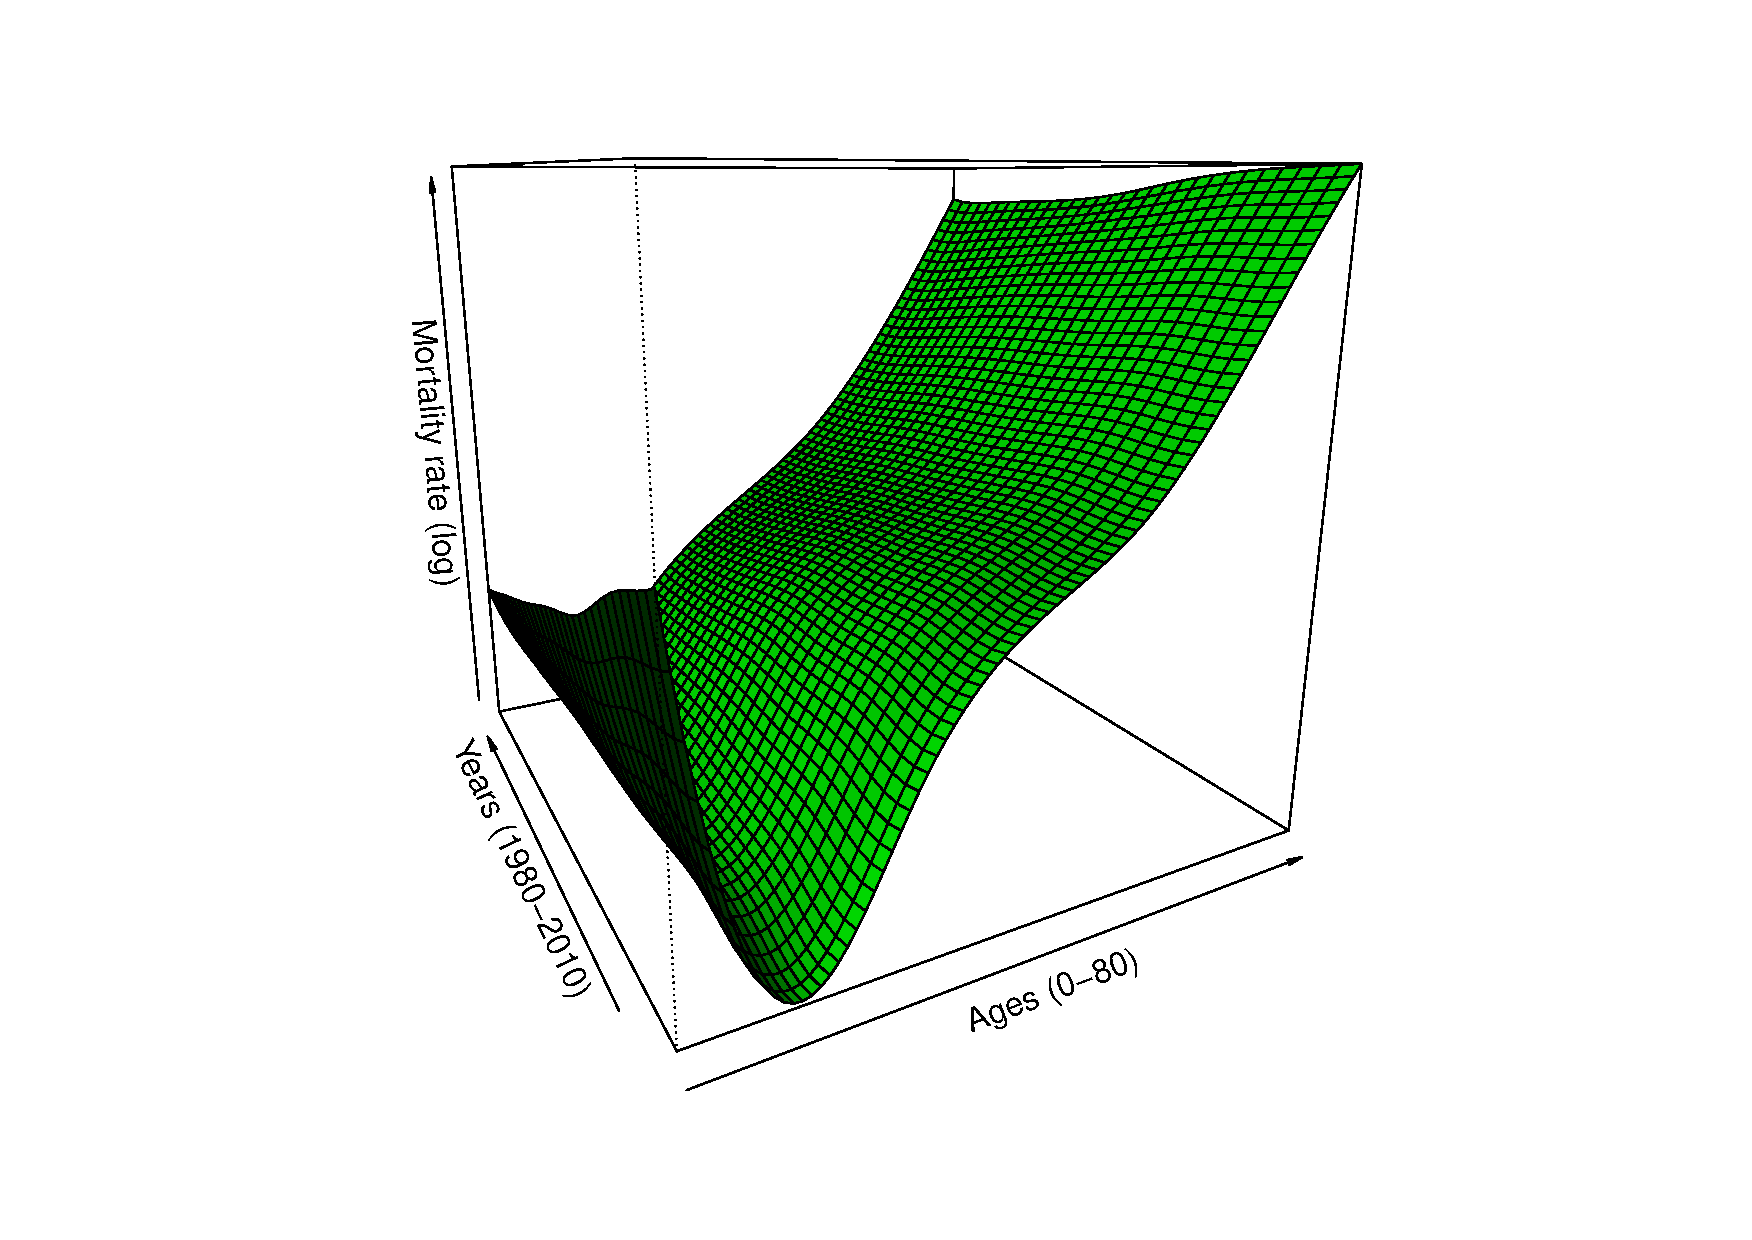
\includegraphics[scale = 0.4]{Graphs/MortalitySurface.pdf}
		\end{center}
		\legend{Fonte: Latin America Human Mortality Database}
		\end{figure} \\
		No eixo referente às idades, observam-se o logarítmo das taxas anuais, para todas as idades. No eixo dos anos é possível ver o comportamento da variável para cada idade \textit{x} durante todo o período. A queda acentuada da mortalidade infantil e para os últimos grupos etários é facilmente observada \cite{brito2008transiccao, brito2010reinvenccao}. Além disso, percebe-se o aumento da mortalidade de jovens adultos durante a década de 80 \cite{araujo1998mortalidade} e a queda das taxas de mortalidade para esse grupo em anos recentes. 
 	\section{Dados de Mercado de Trabalho \label{sec3.2}}
	A principal medida referente ao mercado de trabalho utilizada nesse estudo é a taxa de atividade por idade, definida pelo Instituto Brasileiro de Geografia e Estatística (IBGE) como a porcentagem das pessoas economicamente ativas (PEA), em relação às pessoas de 10 ou mais anos de idade (PIA). Nesse estudo, PEA é definida como os entrevistados com mais de 10 anos de idade que estavam trabalhando, procurando emprego, ou temporariamente afastados de seus trabalhos na semana de referência. \\
	A taxa de atividade para cada idade \textit{x}, denotada como $LFPR_{x}$ é obtida através da razão entre a $PEA_{x}$ e a $PIA_{x}$, na forma da equação~\ref{eq3.5}.
	\begin{equation} \label{eq3.5}
		LFPR_{x} = \dfrac{PEA_{x}}{PIA_{x}}
	\end{equation}
	Os dados necessários para estimar a $LFPR_{x}$ foram obtidos da Pesquisa Nacional por Amostra de Domicílio (PNAD). A PNAD é uma pesquisa amostral, composta por aproximadamente 90.000 domicílios, e realizada anualmente desde 1971, com exceção de 1994 e dos anos nos quais houve realização de censo demográfico. \\
	A pesquisa consiste de dados transversais, e aborda um amplo conjunto de variáveis demográficas e econômicas. A forma detalhada com que os dados são coletados permitiu estimar, de acordo com os critérios aqui estabelecidos, a população economicamente ativa e a população em idade ativa. 
		\subsection{Suavização das Taxas Refinadas de Atividade \label{sec3.2.1}}
		As taxas de atividade estimadas a partir dos dados da PNAD apresentam, para algumas idades, variações que contrariam a tendência global dos dados, de modo que para esse estudo, faz-se necessário ajustar uma curva suavizada.\\
		Suavização é um método que ajusta uma curva aos dados dispostos em um diagrama de dispersão. Essa curva é ajustada de modo que ela possua determinadas propriedades desejáveis, de maneira geral, deseja-se que a curva não apresente variações bruscas, e que ela minimize, localmente, a variância dos resíduos.\\
		O método de suavização utilizado para suavizar as taxas de atividade é conhecida como \textit{LOESS}, que significa \textit{Local Regression} (Regressão Local) \cite{cleveland1979robust, cleveland1988locally}. De maneira intuitiva, a curva ajustada descreve a relação entre duas variáveis de maneira local, ou seja, considerando apenas os pontos mais próximos e não todo o conjunto de dados.
	\section{Modelo Lee--Carter \label{sec3.3}}
	Proposto por \citeonline{lee1992modeling} o modelo Lee--Carter  tem sido amplamente aplicado em demografia e atuária como um modelo estocástico para projeção de taxas de mortalidade. \cite{alonso2015forecasting, mitchell2013modeling, cocco2012longevity}\\
	De acordo com \citeonline{li2009uncertainty}, uma das vantagens do modelo Lee--Carter é que o número de parâmetros a serem estimados são poucos quando comparados com outros modelos estocásticos de mortalidade. Ainda segundo os autores, a estrutura parcimoniosa do modelo garante que  o padrão das taxas de mortalidade por idade não seja contraintuitivo nas projeções. \\
	O modelo tem como objetivo descrever uma superfície de taxas específicas de mortalidade $m_{x,t}$ ou $ln(m_{x,t})$ em função dos parâmetros $a$, $b$ e $k$ de modo a permitir a projeção dessas taxas específicas. Os dois primeiros parâmetros estão relacionados às idades e o último ao tempo. O modelo é descrito pela equação~\ref{eq3.6}:
	\begin{equation} \label{eq3.6}
		ln(m_{x,t}) = a_{x} + b_{x}k_{t} + \epsilon_{x,t}
	\end{equation}
	A equação~\ref{eq3.6} admite infinitas soluções, então $b$ e $k$ devem ser tais que: $\sum_{x}b_{x} = 1$ e $\sum_{t}k_{t} = 0$. Atendidas essas restrições, $a$ é definido simplesmente como a média aritmética de $ln(m_{x,t})$. O vetor $a$ pode ser interpretado como um perfil etário médio, $k$ indica as mudanças no nível de mortalidade ao longo do tempo, e $b$ mostra o efeito da tendência de $k$ para cada grupo etário. \\
	Os valores de $b$ e $k$ foram estimados utilizando mínimos quadrados. Especificamente, os valores de $b$ e $k$ foram estimados através de SVD (Singular Value Decomposition). \\
	O próximo passo envolve utilizar um modelo ARIMA(0,1,0), também chamado de passeio aleatório com drift, para a projeção de $k_{t}$, o que permite observar a tendência esperada para o nível de mortalidade para o período de projeção.
	\begin{equation} \label{eq3.7}
		k_{t} = k_{t-1} + c + \epsilon_{t} 
	\end{equation}
	A equação~\ref{eq3.7} descreve o modelo ARIMA(0,1,0) ajustado para $k_{t}$. Uma vez calculados os valores de $k_{t}$ para o período de projeção basta substituir esses valores na equação~\ref{eq3.6} para obter as taxas específicas de mortalidade.
		\subsection{Modelo Lee-Carter para projeção de Taxas de Atividade \label{sec3.3.1}}
		Para a análise da tendência futura das taxas de atividade, é essencial definir a técnica utilizada para a sua projeção. A metodologia atualmente adotada pelo Ministério da Previdência Social para projeção da PEA, tem suas limitações. \\
		Um dos principais problemas da metodologia atualmente adotada é que as  hipóteses utilizadas integram o modelo, fazendo com que as variáveis estejam relacionadas \cite{schwarzer2009projeccoes}. \\
		As restrições do modelo atualmente utilizado para a realização das projeções do orçamento previdenciário implicam na manutanção dos níveis atuais das taxas de atividade durante todo o horizonte de projeção \cite{projeccao}. Esse estudo propõe a projeção das taxas de atividade utilizando do modelo Lee--Carter. A simplicidade do modelo, e o fato de que ele utiliza a série histórica das taxas para a previsão são as principais razões que levaram a sua escolha como uma maneira alternativa de realizar a projeção. \\
		Seguindo a abordagem adotada por \citeonline{rodrigues2010analise} para projeção de taxas de utilização de serviços de saúde, a matriz de taxas específicas de mortalidade $ln(m_{x,t})$ passa a ser definida como uma matriz de taxas de atividade, denotada por $ln(LFPR_{x,t})$. Os resultados são apresentados na seção~\ref{sec4.2}.
	\section{A duração esperada da Aposentadoria (ELRP) \label{sec3.4}}
	De acordo com \citeonline{lee2001expected}, se um homem se aposenta com \emph{x} anos de idade, é natural assumir que a sua aposentadoria tenha a mesma duração de $e_{x}$, sua expectativa de vida, assim, dentre os membros de uma coorte, a proporção de pessoas que teriam sua aposentadoria com duração $e_{x}$ é igual à probabilidade de se aposentar com \emph{x} anos de idade. Tendo isso em mente, a duração esperada da aposentadoria pode ser definida como uma média ponderada da expectativa de vida a cada idade de aposentadoria \emph{x}. \\
	O peso associado a $e_{x}$ é a probabilidade de aposentadoria, definida como o produto de $S_{x}$, (probabilidade de permanecer vivo até a idade \emph{x}), $T_{x}$, (probabilidade de se manter no mercado de trabalho até a idade \emph{x}) e $\gamma_{x}$, (probabilidade de se aposentar à idade \emph{x}). Dentre os homens que se aposentariam no intervalo [\emph{x}, \emph{x+1}), a proporção dos que morrem antes da aposentadoria é dada por $q_{x}$, assumindo que a probabilidade de aposentadoria é constante no intervalo etário, metade dos homens morrem antes de se aposentarem, ou seja, a probabilidade de aposentadoria no intervalo [\emph{x}, \emph{x+1}) passa a ser definida como: $S_{x}T_{x}\gamma_{x}[1-(0,5q_x)]$. Adicionalmente, se um homem se aposenta durante o intervalo [\emph{x}, \emph{x+1})  a duração esperada da sua aposentadoria é $(e_{x}+e_{x+1})/2$. Logo, a duração esperada da aposentadoria é definida pela equação:
	\begin{equation} \label{eq4.1}
		ELRP = \sum_{x=20}^{80}S_{x}T_{x}\gamma_{x}[1-(0,5q_x)]\left[\dfrac{(e_x + e_{x+1})}{2}\right]
	\end{equation}
	A equação~\ref{eq4.1} pode ser reescrita, de maneira equivalente, como:
	\begin{equation} \label{eq4.2}
		ELRP = \rho^{20-50}\sum_{x=50}^{80}S_{x}T_{x}\gamma_{x}[1-(0,5q_x)]\left[\dfrac{(e_x + e_{x+1})}{2}\right]
	\end{equation}
onde $\rho^{20-50}$ é a probabilidade de sobreviver ao intervalo etário [20,50). A equação~\ref{eq4.2} tem como principal objetivo simplificar os cálculos, para trabalhar com essa simplificação, é necessário assumir que a saída permanente do mercado de trabalho ocorre com uma frequência significativa a partir dos 50 anos. \\
	Destaca-se que as estimativas encontradas neste estudo são baseadas em tábuas de vida de período, então, assume-se que a duração da aposentadoria de um homem de 20 anos é calculada com base nos níveis de mortalidade e de participação no mercado de trabalho atuais. Essa estimativa é subestimada, uma vez que este homem vai experimentar em sua vida, níveis de mortalidade e de participação no mercado de trabalho diferentes do que os utilizados no cálculo.
%---

%---
% Resultados

\chapter{Resultados \label{cap4}}
	\section{Evolução das Taxas de Mortalidade \label{sec4.1}}
	Após o ajuste do modelo Lee--Carter é essencial fazer uma análise gráfica com o objetivo de validar a adequação aos dados. O primeiro passo é avaliar os gráficos dos parâmetros $a$ e $b$, que indicam, respectivamente, o perfil da curva de mortalidade por idade e o padrão dos desvios do perfil da curva de mortalidade de acordo com a variação de \textit{k}, a figura~\ref{fig2} apresenta gráficos para esses dois parâmetros. Nessa análise, destacam-se o aumento do nível de mortalidade para jovens adultos, consequência do aumento no nível de mortalidade por causas externas para essas idades, principalmente durante a década de 80 \cite{araujo1998mortalidade}, e a acentuada queda das taxas de mortalidade infantil, resultado do processo de transição demográfica \cite{brito2008transiccao}.\\
 	\begin{figure}[!htb]
	\caption{\label{fig2} Parâmetros \textit{a} e \textit{b} do modelo Lee--Carter}
		\begin{subfigure}[b]{0.5\textwidth}
		\begin{center}
			\caption{\label{fig2.1} Parâmetro \textit{a}}
			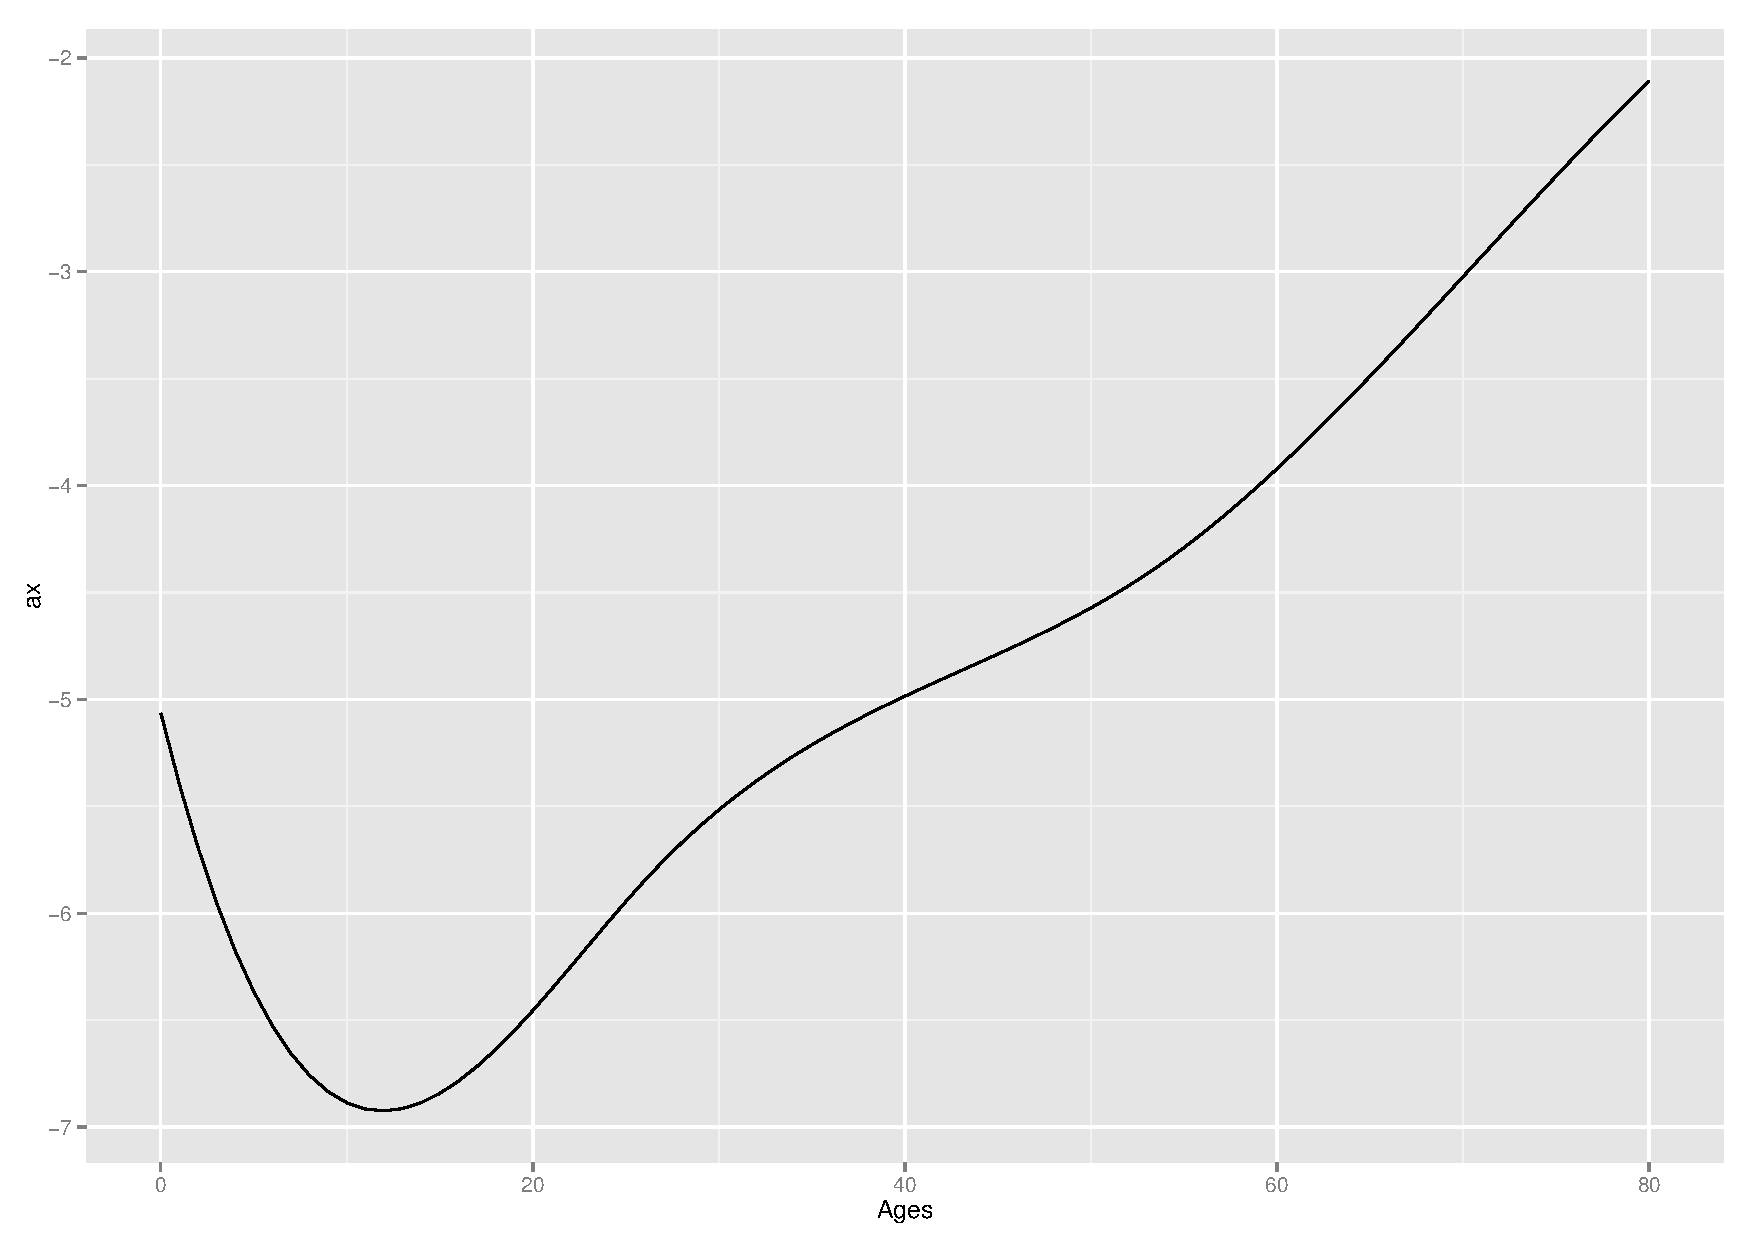
\includegraphics[width=\textwidth]{Graphs/DR_LC_ax.pdf}
		\end{center}
		\end{subfigure}
	\hfill
		\begin{subfigure}[b]{0.5\textwidth}
		\begin{center}
			\caption{\label{fig2.2} Parâmetro \textit{b}}
			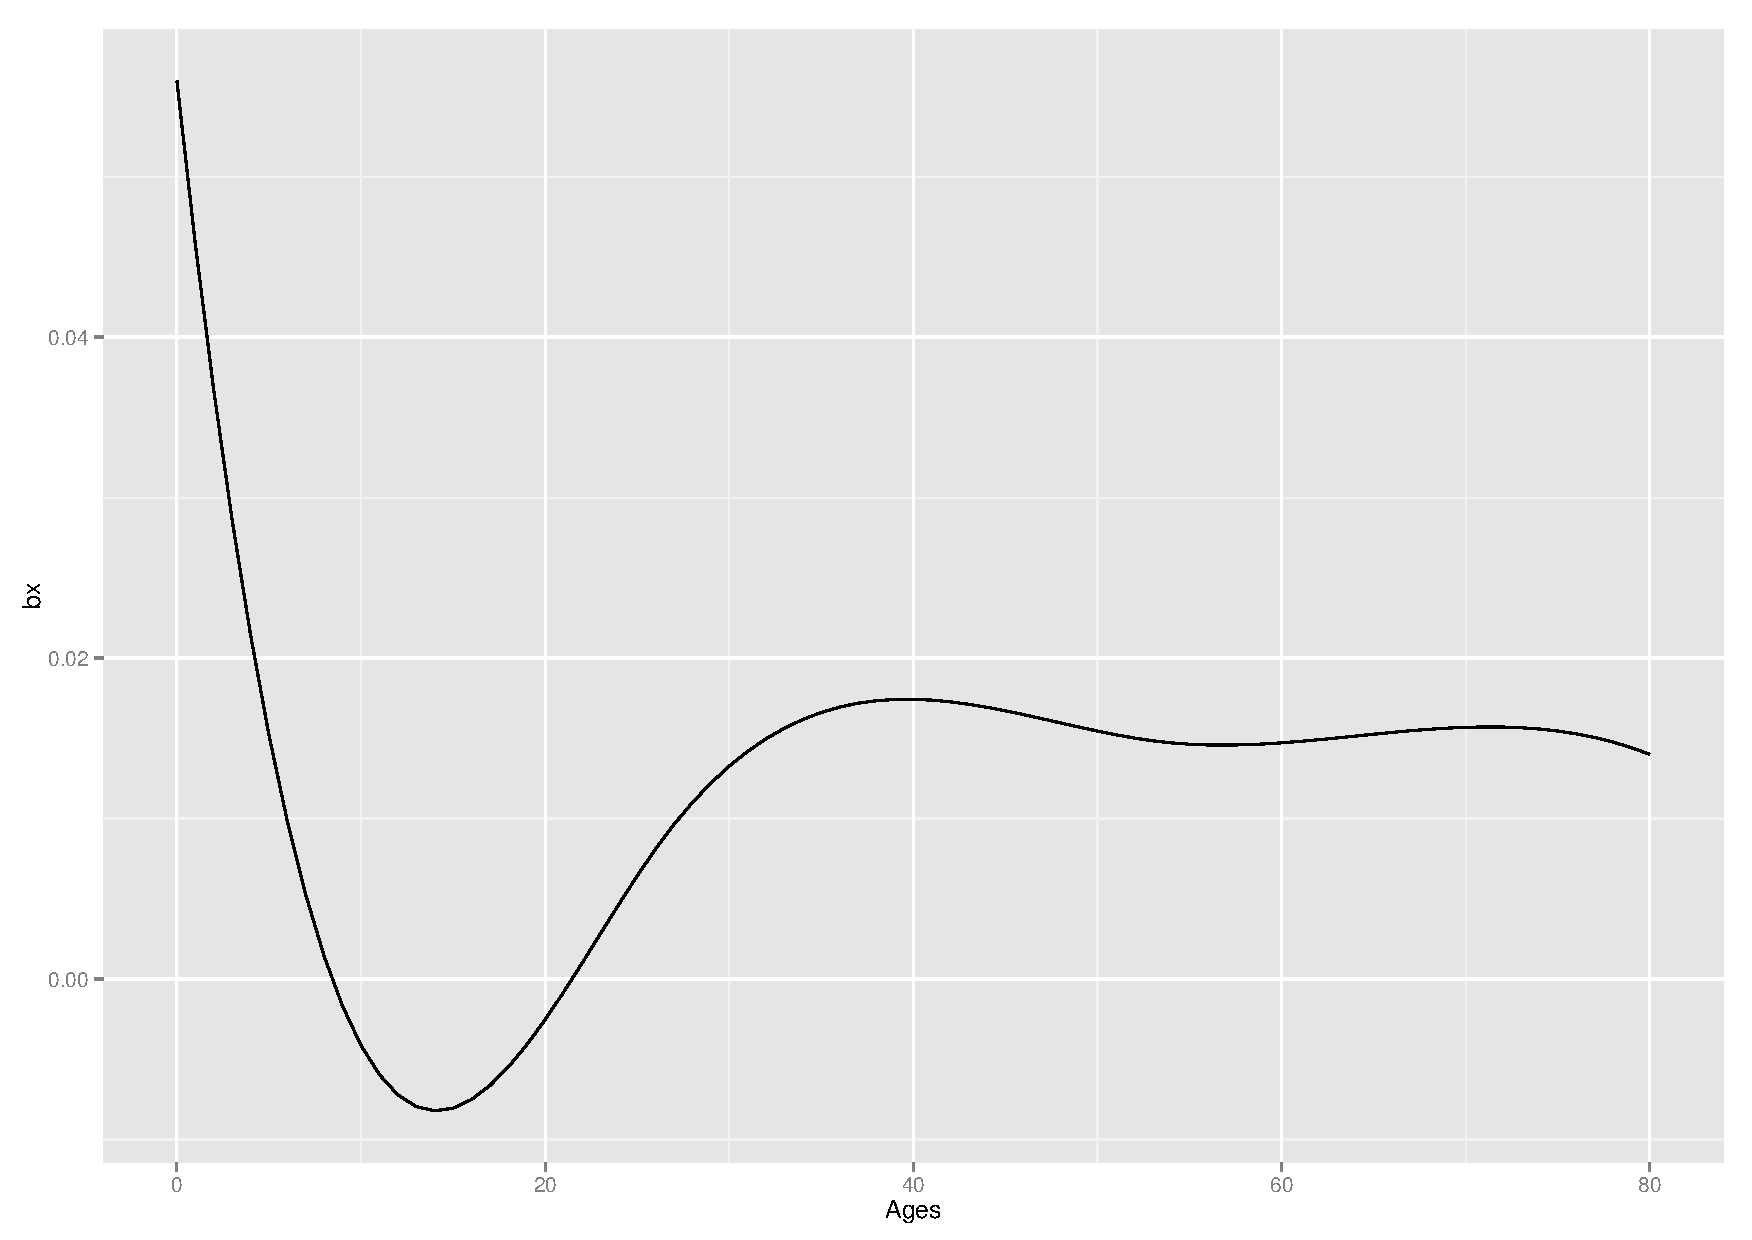
\includegraphics[width=\textwidth]{Graphs/DR_LC_bx.pdf}
		\end{center}
 		\end{subfigure}
	\legend{Fonte: Latin America Human Mortality Database}
	\end{figure} \\
	Destaca-se também que a figura~\ref{fig2.1} apresenta o formato padrão de curvas definidas por $f(x) = ln(m_{x})$, com um baixo nível de mortalidade nas primeiras idades e com tendência crescente a partir dos 20 anos de idade. \\
	O comportamento do parâmetro \textit{k} indica a tendência observada para o nível das taxas de mortalidade para todas as idades. Observa-se que o parâmetro apresenta uma tendência de queda para todo o período observado, e como resultado disso, o modelo apresenta estimativas para o período de projeção que seguem essa mesma tendência. A figura~\ref{fig3} apresenta intervalos de confiança com nível de confiança $\alpha= 0,95$ para as estimativas de \textit{k}, como o parâmetro apresenta uma tendência constante de queda, os intervalos estimados são bastante estreitos. \\
	\begin{figure}[!htb]
	\caption{\label{fig3} Parâmetro \textit{k}}
		\begin{center}
			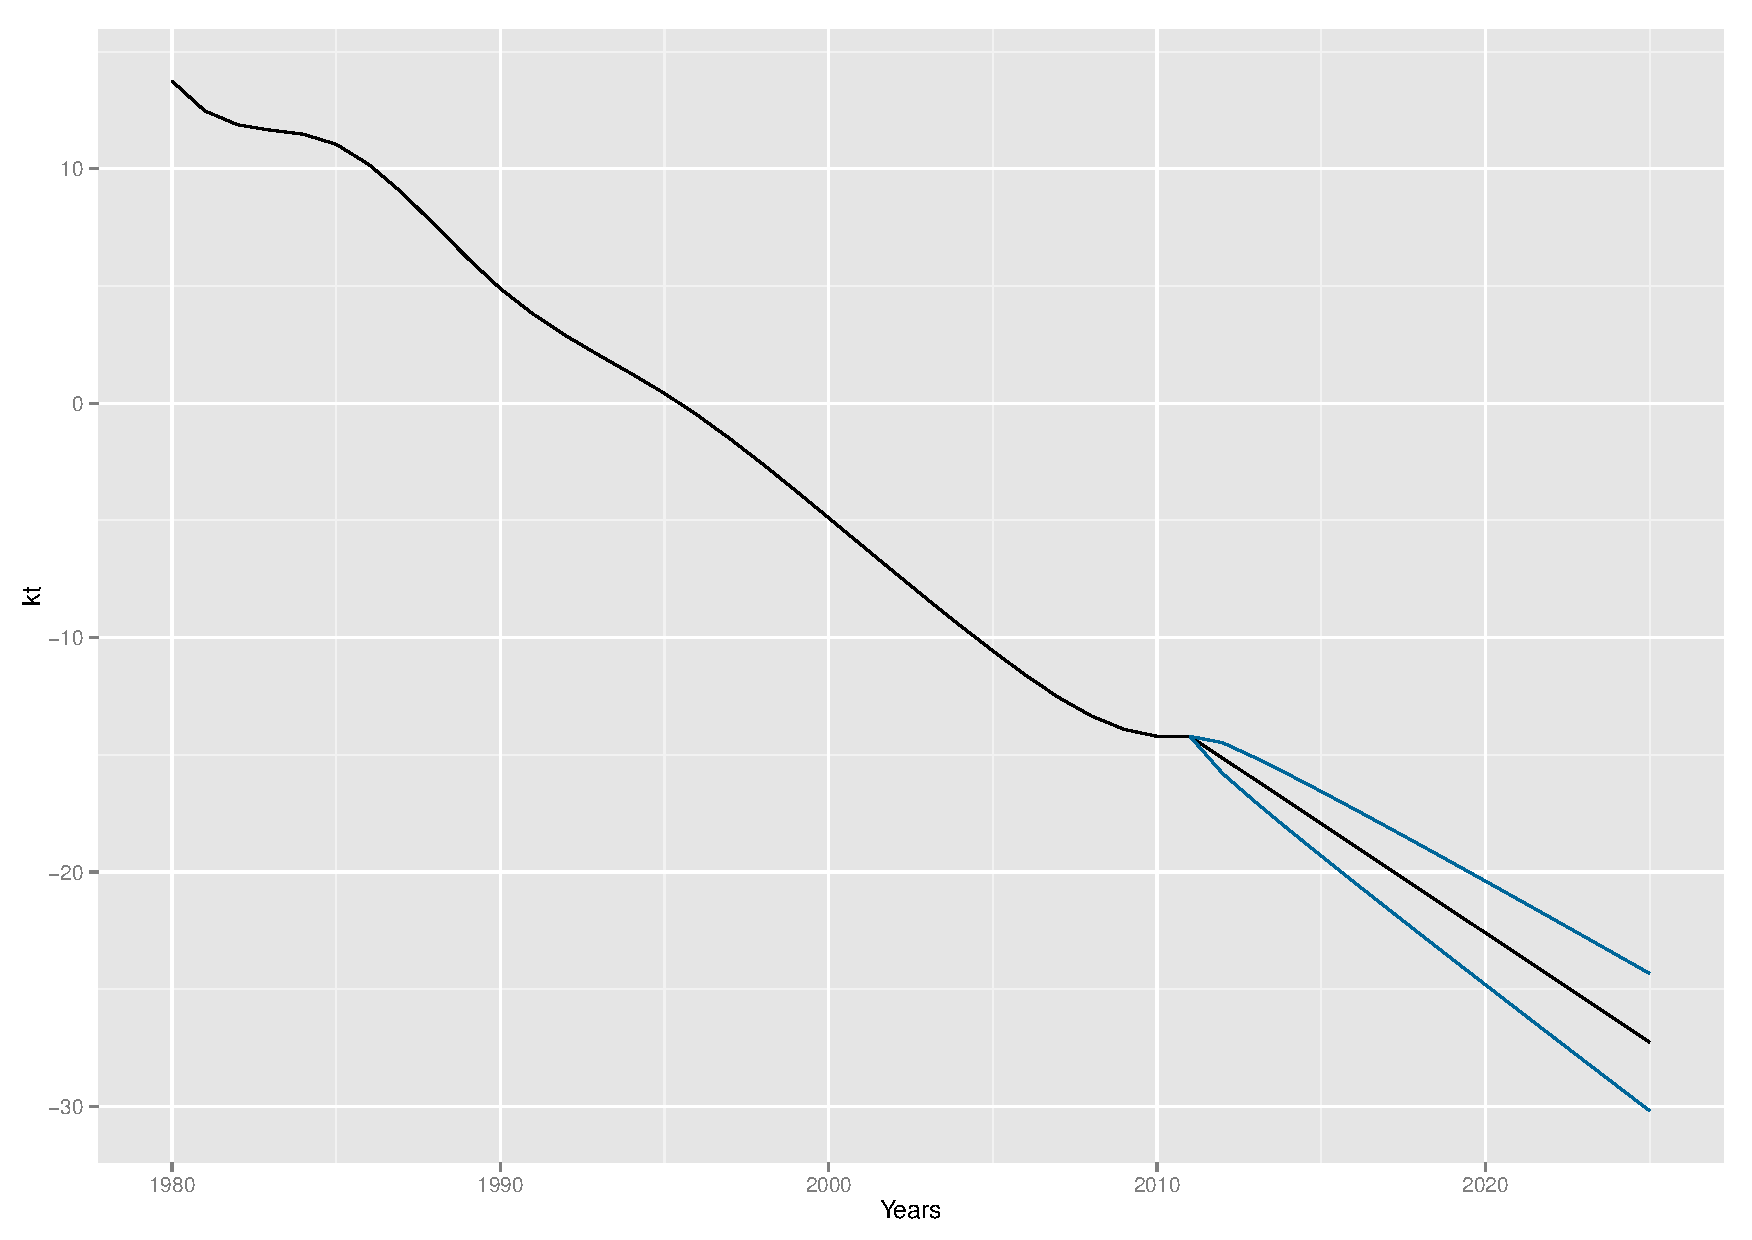
\includegraphics[scale = 0.35]{Graphs/DR_LC_kt_f.pdf}
		\end{center}
	\legend{Fonte: Latin America Human Mortality Database}
	\end{figure} \\
	Para medir a capacidade do modelo de projetar taxas de mortalidade, o modelo foi ajustado novamente, mas considerando uma série histórica sem os dados dos últimos doze anos, e comparada com os dados observados naquele ano. A figura~\ref{fig4.1} apresenta a comparação entre as taxas de mortalidade projetadas e reais e a figura~\ref{fig4.2} as taxas projetadas para anos selecionados. \\
	\begin{figure}[!htb]
	\caption{\label{fig4} Validação do Modelo e Taxas projetadas}
		\begin{subfigure}[b]{0.5\textwidth}
		\begin{center}
			\caption{\label{fig4.1} Lee--Carter e Observado}
			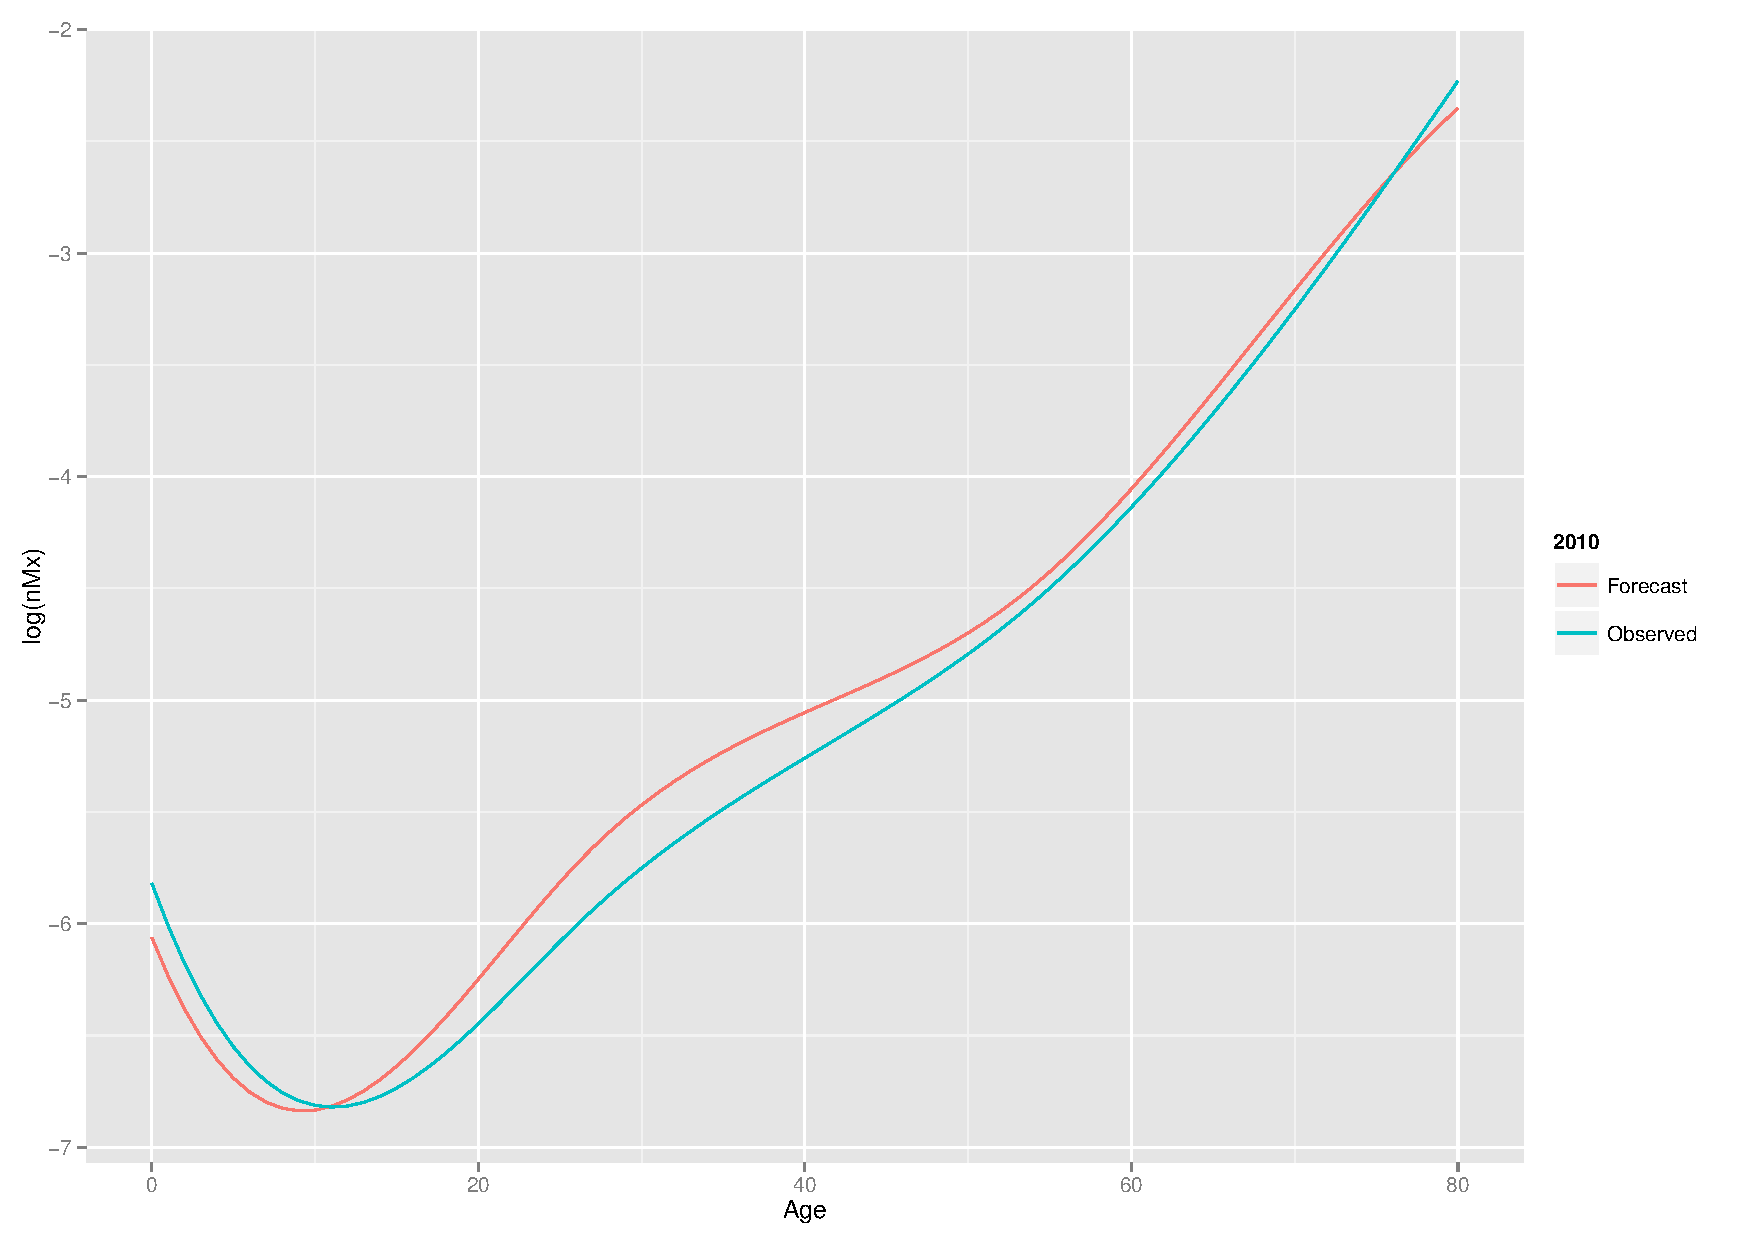
\includegraphics[width=\textwidth]{Graphs/DR_validation.pdf}
		\end{center}
		\end{subfigure}
	\hfill
		\begin{subfigure}[b]{0.5\textwidth}
		\begin{center}
			\caption{\label{fig4.2} $ln(m_{x})$ - Anos Selecionados}
			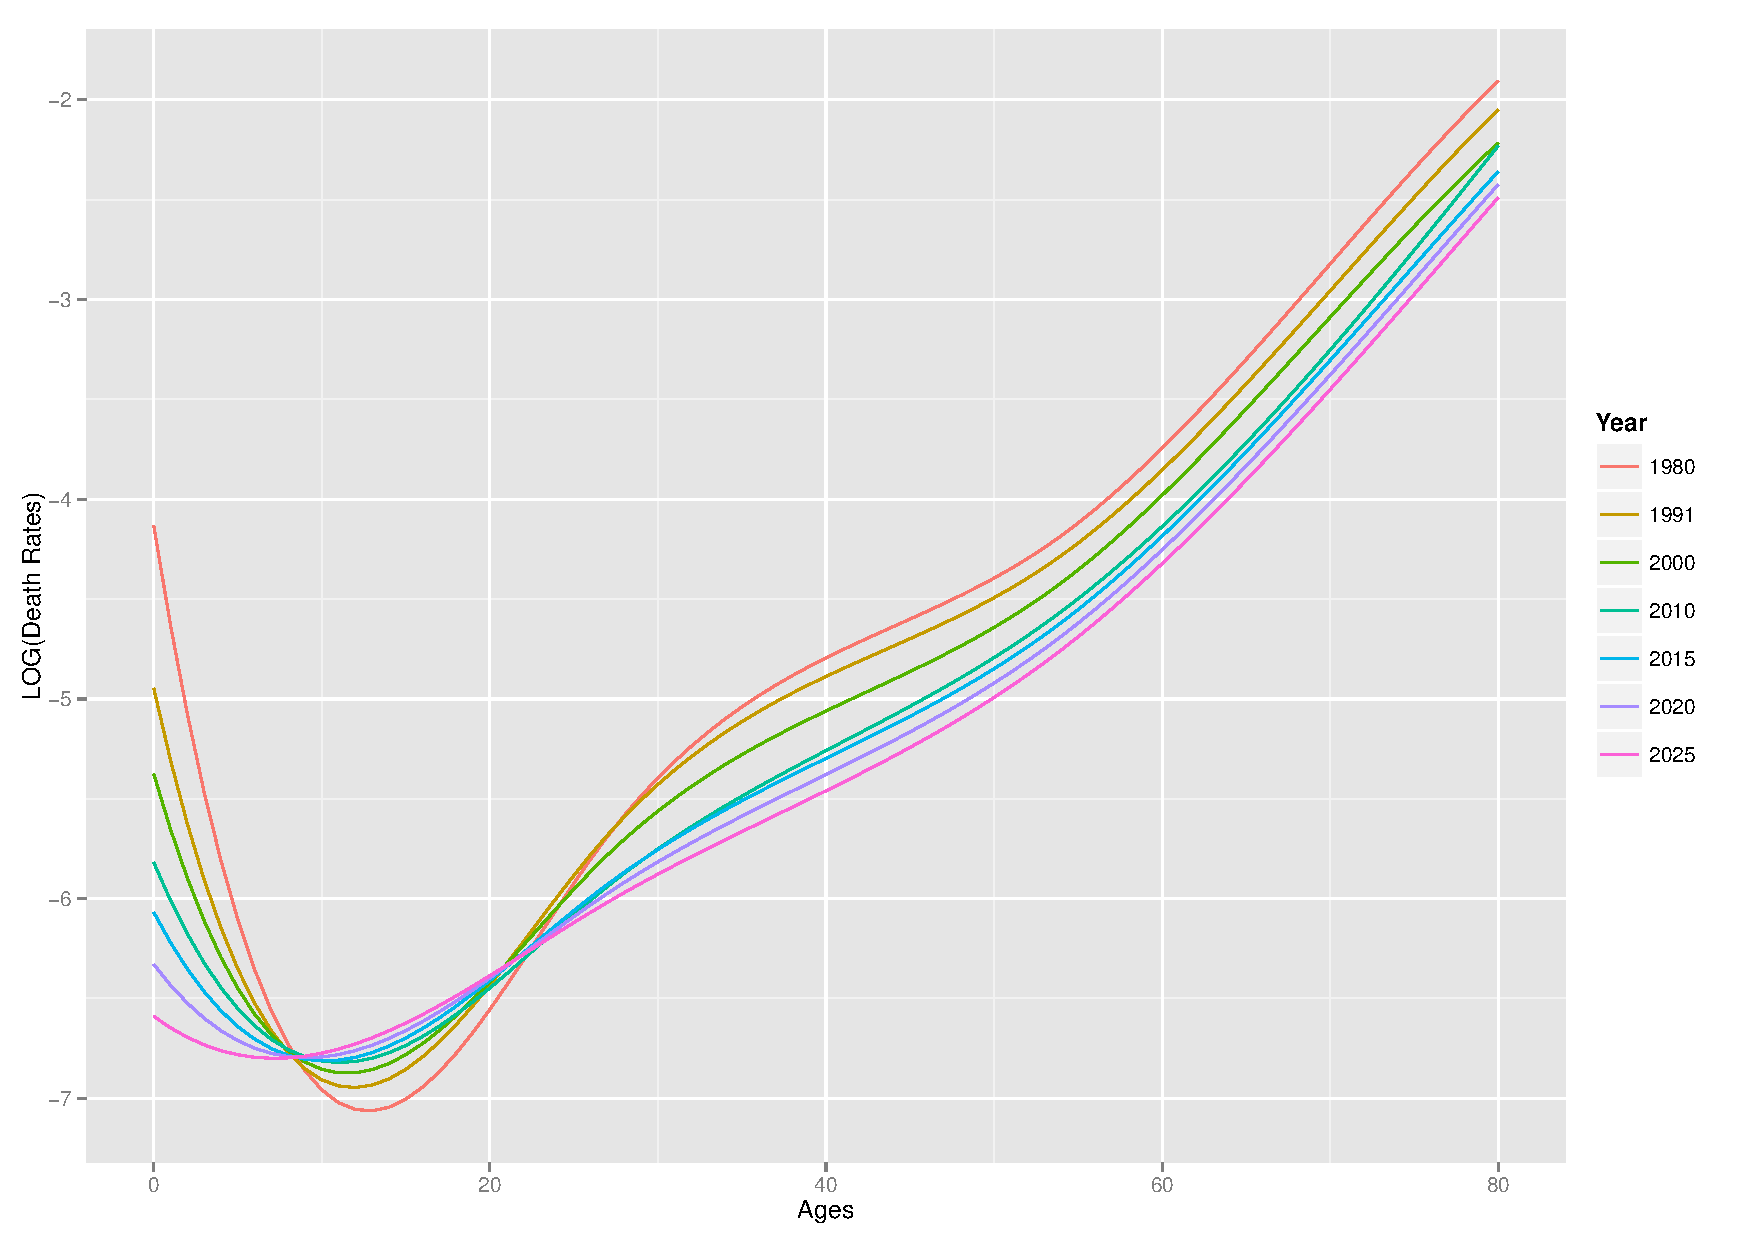
\includegraphics[width=\textwidth]{Graphs/DR_select.pdf}
		\end{center}
 		\end{subfigure}
	\legend{Fonte: Latin America Human Mortality Database}
	\end{figure} \\
	Considerando que o período utilizado para o teste de validação tem início em 1980 e termina em 1996, um período curto para realizar projeções, o descolamento observado na figura~\ref{fig4.1} é explicado pela queda acentuada da mortalidade infantil e o aumento das mortes de jovens adultos por causas externas observado no período \cite{waiselfisz2011mapa, duarte2012associaccao, carvalho2012bayesian}. Além disso, como apresentado na seção~\ref{sec3.3}, para que a equação~\ref{eq3.6} tenha um número finito de soluções, $b$ é tal que $\sum_{x}b_{x} = 1$, então, a queda acentuada na mortalidade infantil afeta o formato da curva nas demais idades.\\
	A figura~\ref{fig4.2} mostra a evolução esperada das taxas de mortalidade estimadas pelo modelo, considerando o período, destaca-se que o modelo estima que o nível das taxas de mortalidade para jovens adultos será mais alto do que o observado atualmente, isso é consequência direta da distorção ocorrida na estimação do parâmetro \textit{b} (figura~\ref{fig2.2}). \\
	Apesar da ressalva com relação ao ajuste do modelo para projetar taxas de mortalidade para as primeiras idades, o modelo foi considerado adequado considerando o grupo etário em estudo. Logo, as taxas projetadas para o período 2014-2025 são utilizadas para o cálculo da duração esperada da aposentadoria.
	\section{Evolução das Taxas de Atividade \label{sec4.2}}
	Esse estudo propõe o uso do modelo Lee--Carter para projeção das taxas de atividade, tendo em mente que o modelo original não foi construído com esse objetivo, faz-se necessário uma avaliação criteriosa do ajuste do modelo. A utilização de um modelo estocástico permite incorporar as mudanças recentes no nível da taxa de atividade, as projeções. A figura~\ref{fig5} apresenta os gráficos dos parâmetros $a$ e $b$, que representam medidas do nível das taxas de atividade. \\
	 \begin{figure}[!htb]
	\caption{\label{fig5} Parâmetros \textit{a} e \textit{b} do modelo Lee--Carter}
		\begin{subfigure}[b]{0.5\textwidth}
		\begin{center}
			\caption{\label{fig5.1} Parâmetro \textit{a}}
			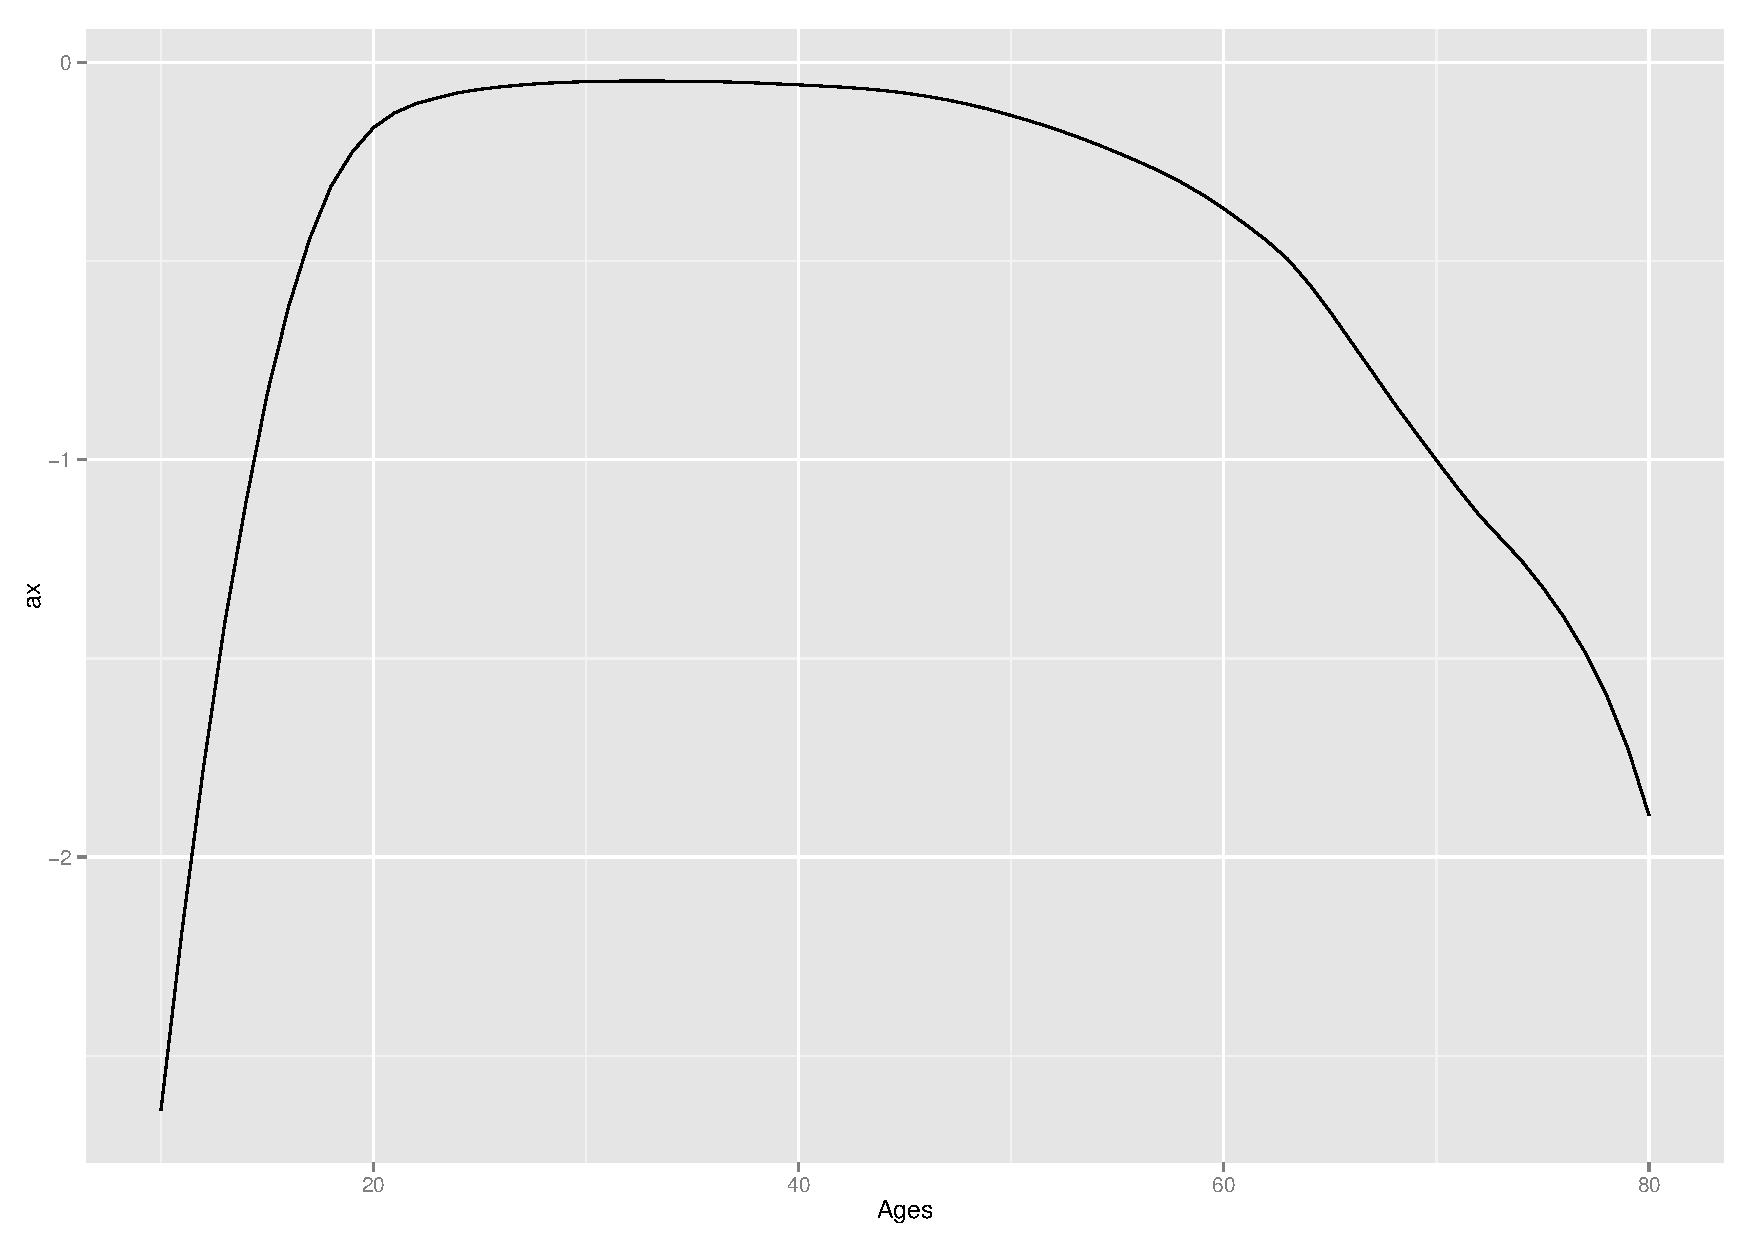
\includegraphics[width=\textwidth]{Graphs/LFPR_LC_ax.pdf}
		\end{center}
		\end{subfigure}
	\hfill
		\begin{subfigure}[b]{0.5\textwidth}
		\begin{center}
			\caption{\label{fig5.2} Parâmetro \textit{b}}
			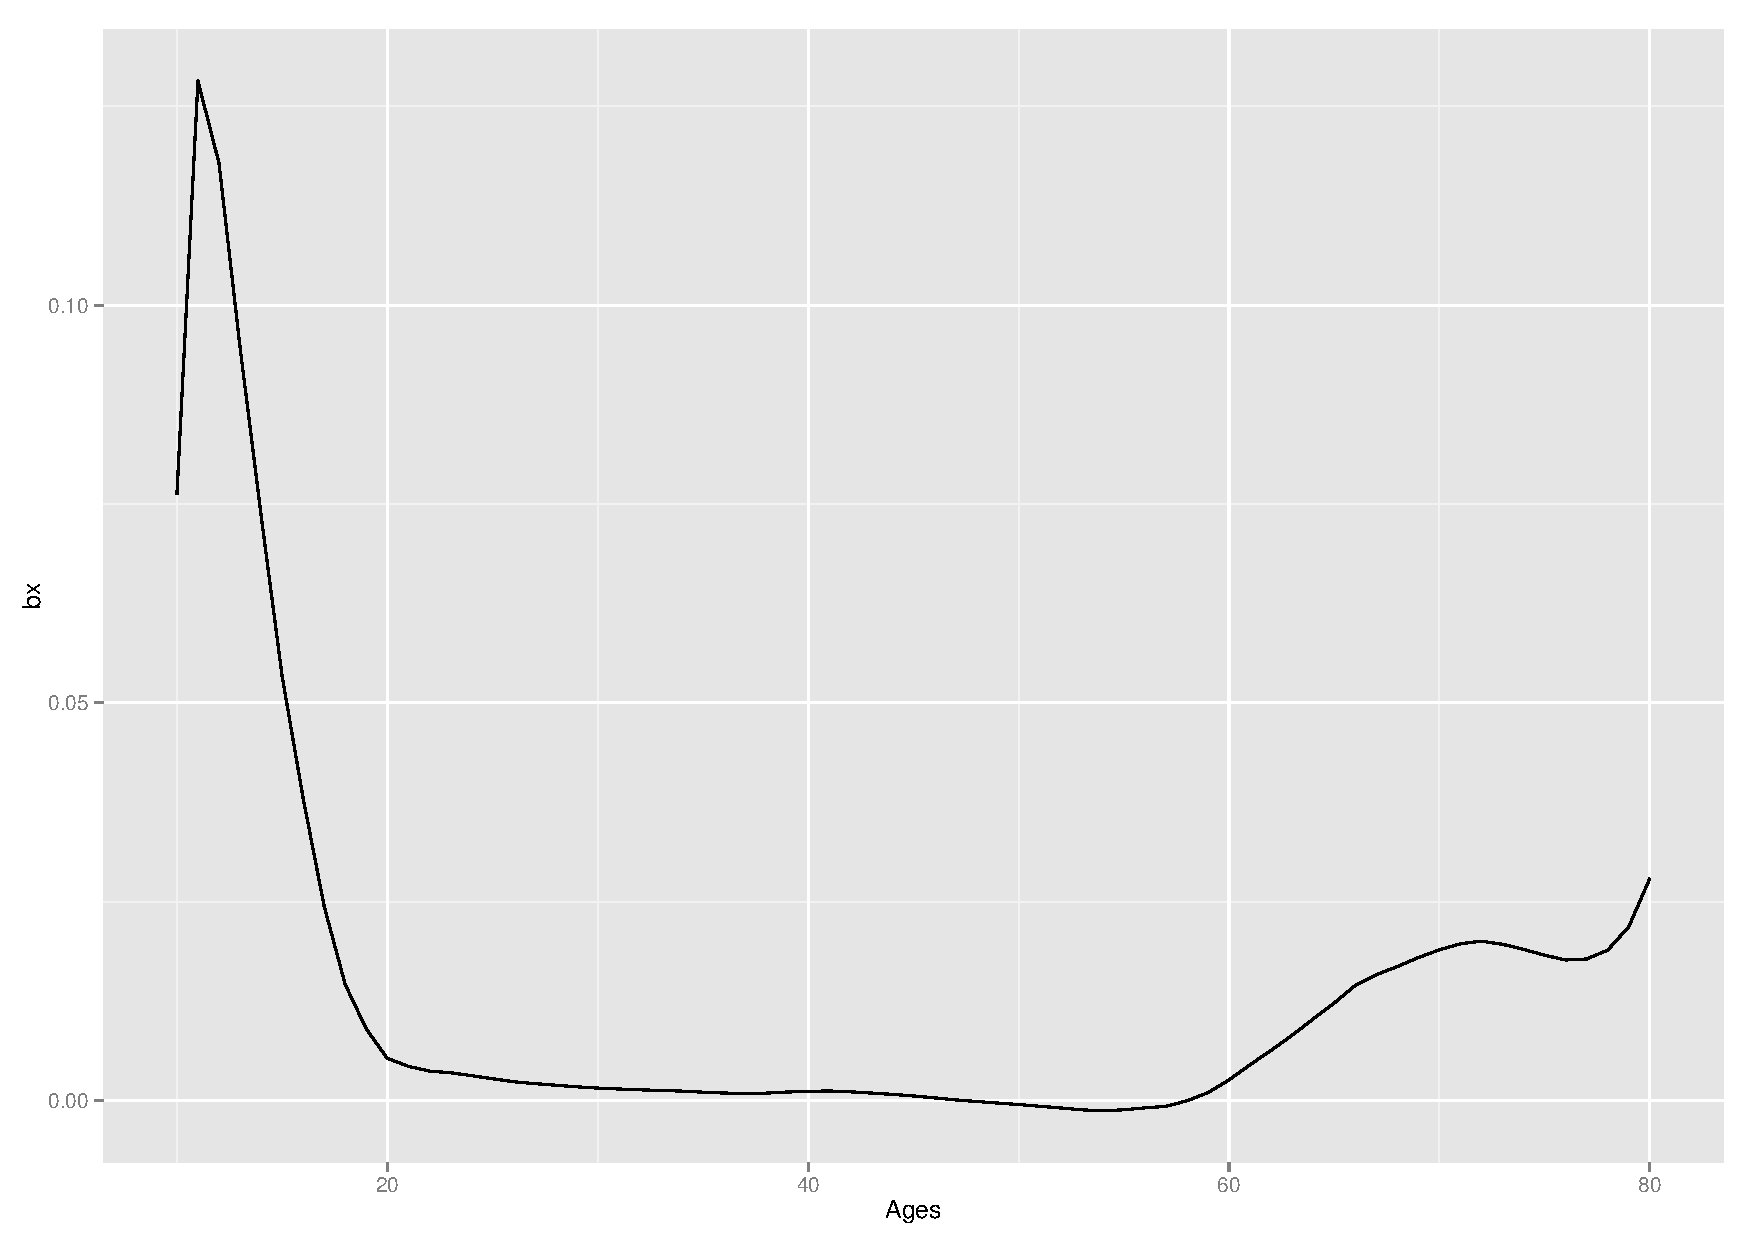
\includegraphics[width=\textwidth]{Graphs/LFPR_LC_bx.pdf}
		\end{center}
 		\end{subfigure}
	\legend{Fonte: PNAD}
	\end{figure} \\
	A figura~\ref{fig5.1} apresenta, em escala logarítmica, o padrão observado para o intervalo entre 1980 e 2013 das taxas de atividade masculinas. O formato da curva apresenta o formato esperado, com taxas de atividade baixas nas primeiras idades, elevadas e razoavelmente constantes durante as idades de 20 a 50 anos, e declinando após essa idade. A figura~\ref{fig5.2} demonstra a suposição mais importante para esse estudo, no que diz respeito a projeção das taxas de atividade, as variações no nível da taxa de participação por idade. Observando o comportamento da curva do parâmetro $b$, dois pontos chamam atenção, a queda na taxa de atividade para os primeiros e últimos grupos etários, o que indica uma entrada tardia, e uma saída precoce do mercado de trabalho, respectivamente. Essas tendências, aliadas a queda da mortalidade nas idades mais avançadas (figura~\ref{fig4.2}) impacta diretamente o regime de financiamento do RGPS.
	\begin{figure}[!htb]
	\caption{\label{fig6} Parâmetro \textit{k}}
		\begin{center}
			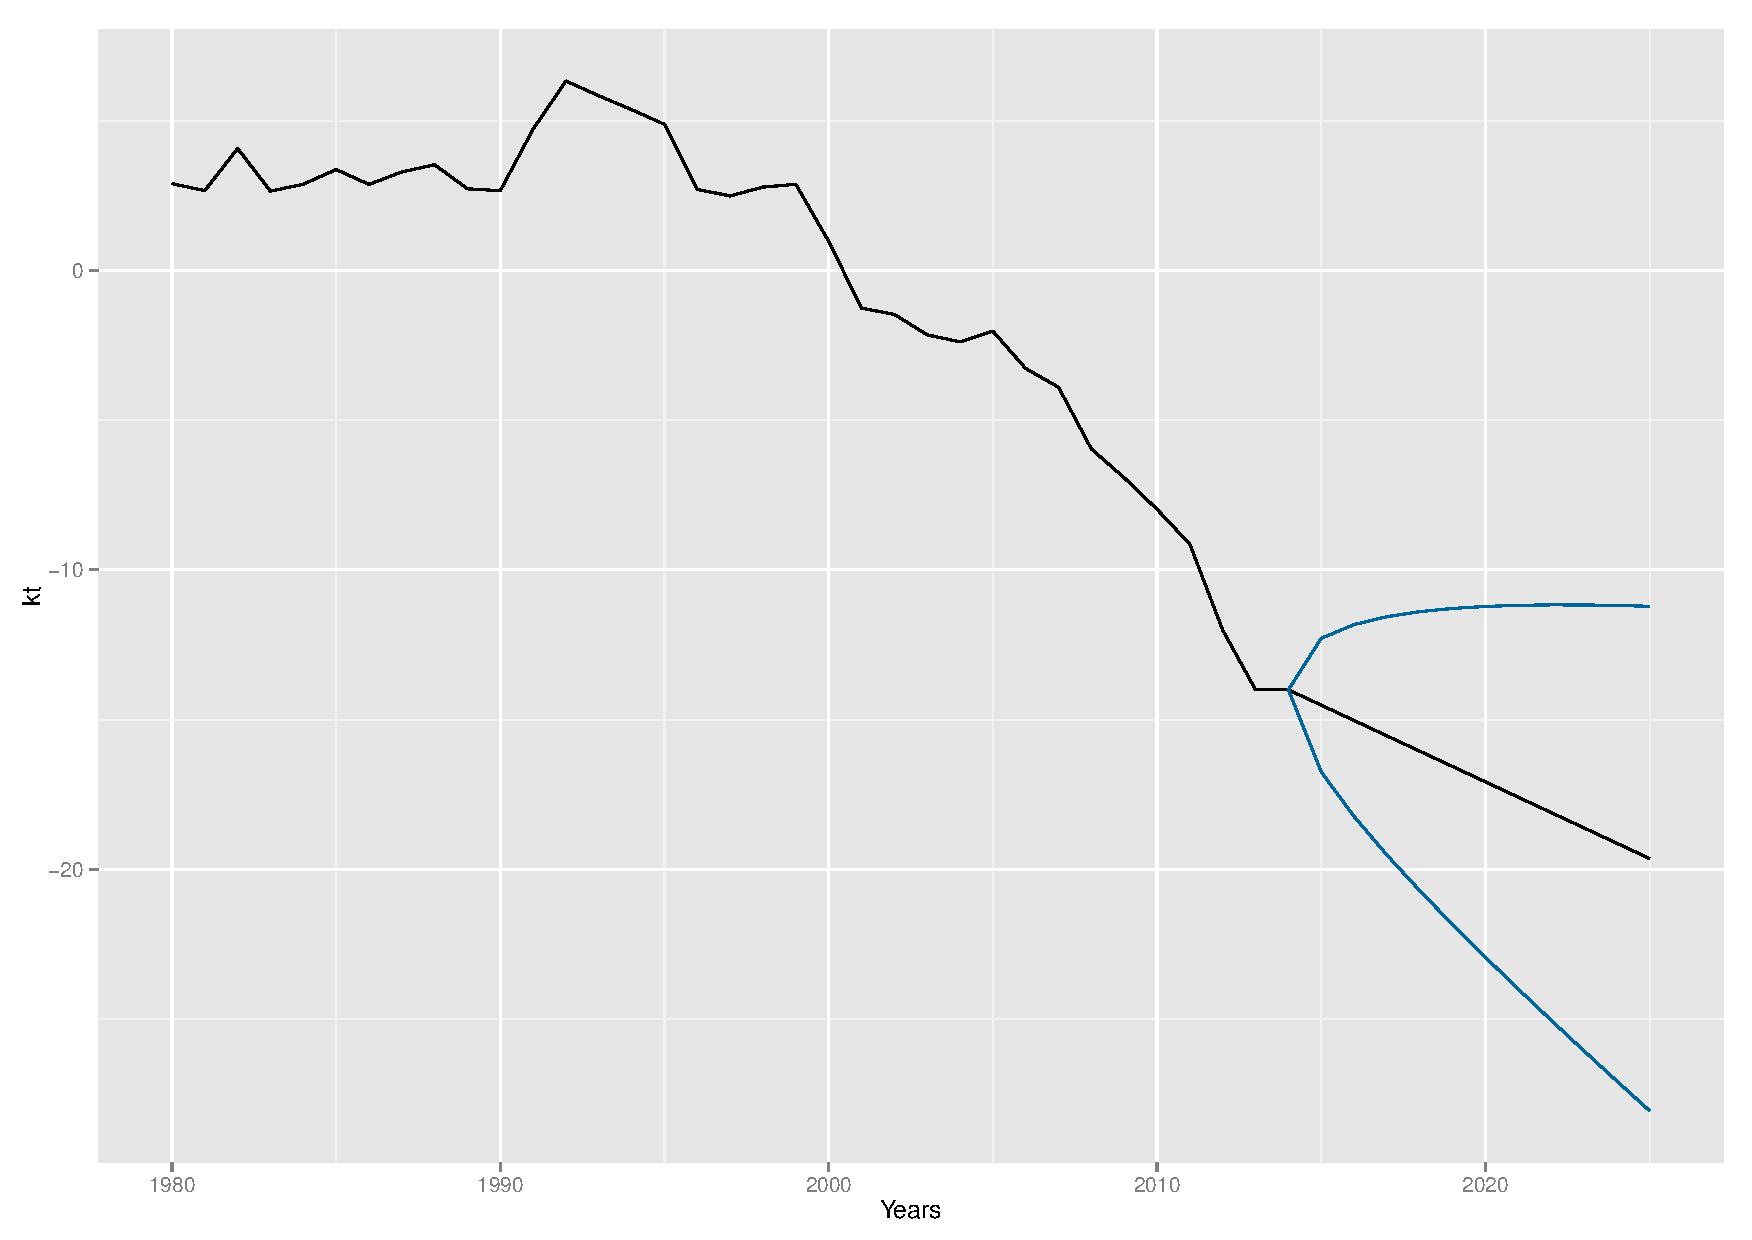
\includegraphics[scale = 0.35]{Graphs/LFPR_LC_kt_f.pdf}
		\end{center}
	\legend{Fonte: PNAD}
	\end{figure} \\
	A figura~\ref{fig6} apresenta a tendência do nível da taxa de atividade, independente do grupo etário, para todos os anos. Observa-se que, durante o período entre 1980-1990 o parâmetro apresenta um comportamento quase que constante, com algumas flutuações. Entre 1990-1991 percebemos um aumento considerável no nível da taxa de atividade, mas a partir desse ponto até o ano de 2013, a tendência de queda é clara. \\
	Destaca-se que para o período de projeção, o intervalo de confiança calculado para o parâmetro não é tão informativo quanto aquele calculado para a taxa de mortalidade. Apesar de os dois intervalos utilizarem o mesmo nível de confiança $\alpha = 0,95$, o comportamento das estimativas do parâmetro $k$ influenciam a amplitude do intervalo. A figura~\ref{fig3} aponta para uma tendência clara de queda em qualquer ponto dentro do intervalo, enquanto o intervalo aqui apresentado é bastante amplo e abriga, no mínimo, três cenários distintos, listados a seguir:
	\begin{itemize}
		\item{queda do nível das taxas de atividade}
		\item{nível constante das taxas de atividade}
		\item{aumento do nível das taxas de atividade}
	\end{itemize}
	Uma maneira de avaliar se as estimativas de $k$ podem ser consideradas razoáveis apesar da amplitude do intervalo de confiança é realizar a validação do modelo, esse procedimento permite comparar as taxas observadas com as projeções para um determinado ano. A figura~\ref{fig7.1} apresenta as taxas de atividade por idade observadas e projetadas para o ano de 2013, observa-se que o modelo apresenta um ajuste muito próximo dos dados reais. Dessa forma, o modelo Lee--Carter parece ser uma alternativa confiável para a projeção de taxas de atividade, principalmente pela capacidade de incorporar a tendência de queda no nível das taxas. \\
	\begin{figure}[!htb]
	\caption{\label{fig7} Validação do Modelo e Taxas projetadas}
		\begin{subfigure}[b]{0.5\textwidth}
		\begin{center}
			\caption{\label{fig7.1} Lee--Carter e Observado}
			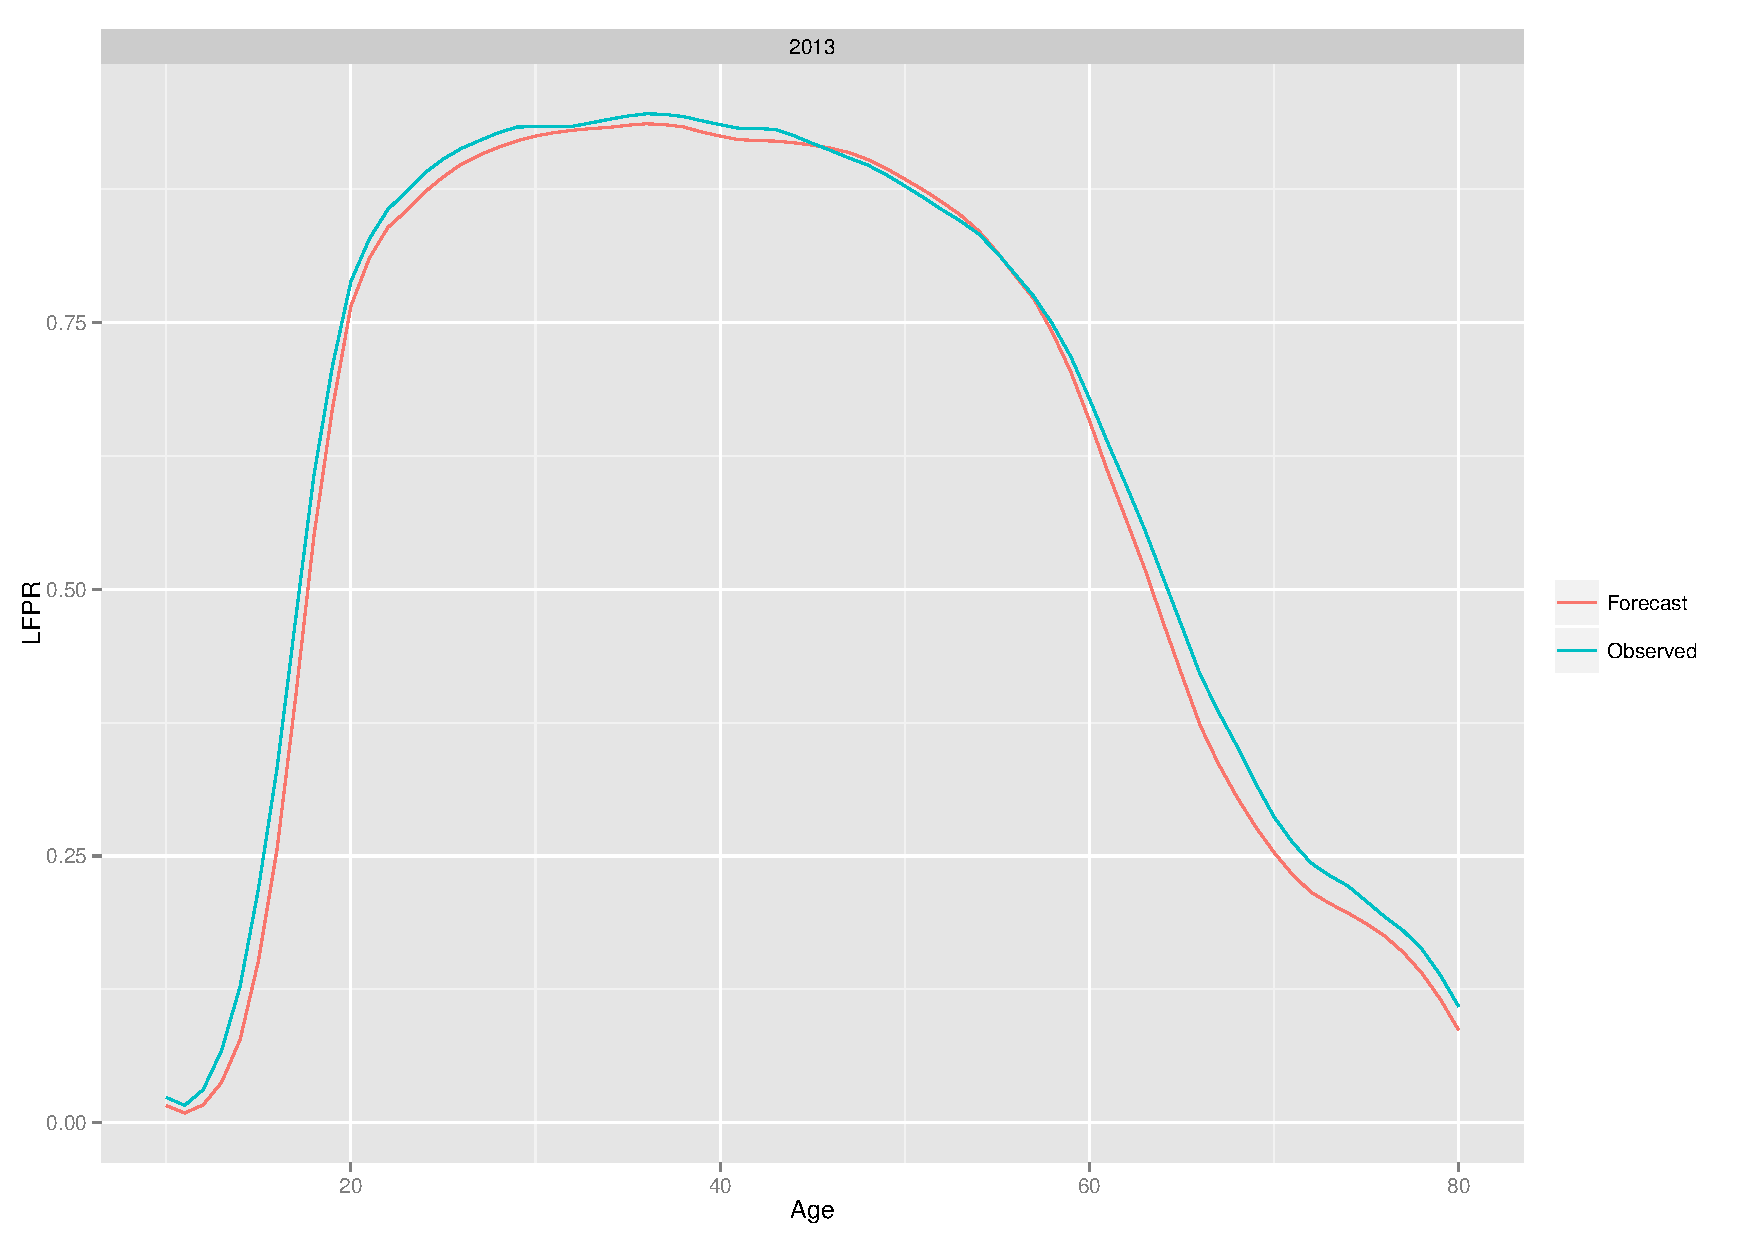
\includegraphics[width=\textwidth]{Graphs/LFPR_validation.pdf}
		\end{center}
		\end{subfigure}
	\hfill
		\begin{subfigure}[b]{0.5\textwidth}
		\begin{center}
			\caption{\label{fig7.2} $ln(LFPR_{x})$ - Anos Selecionados}
			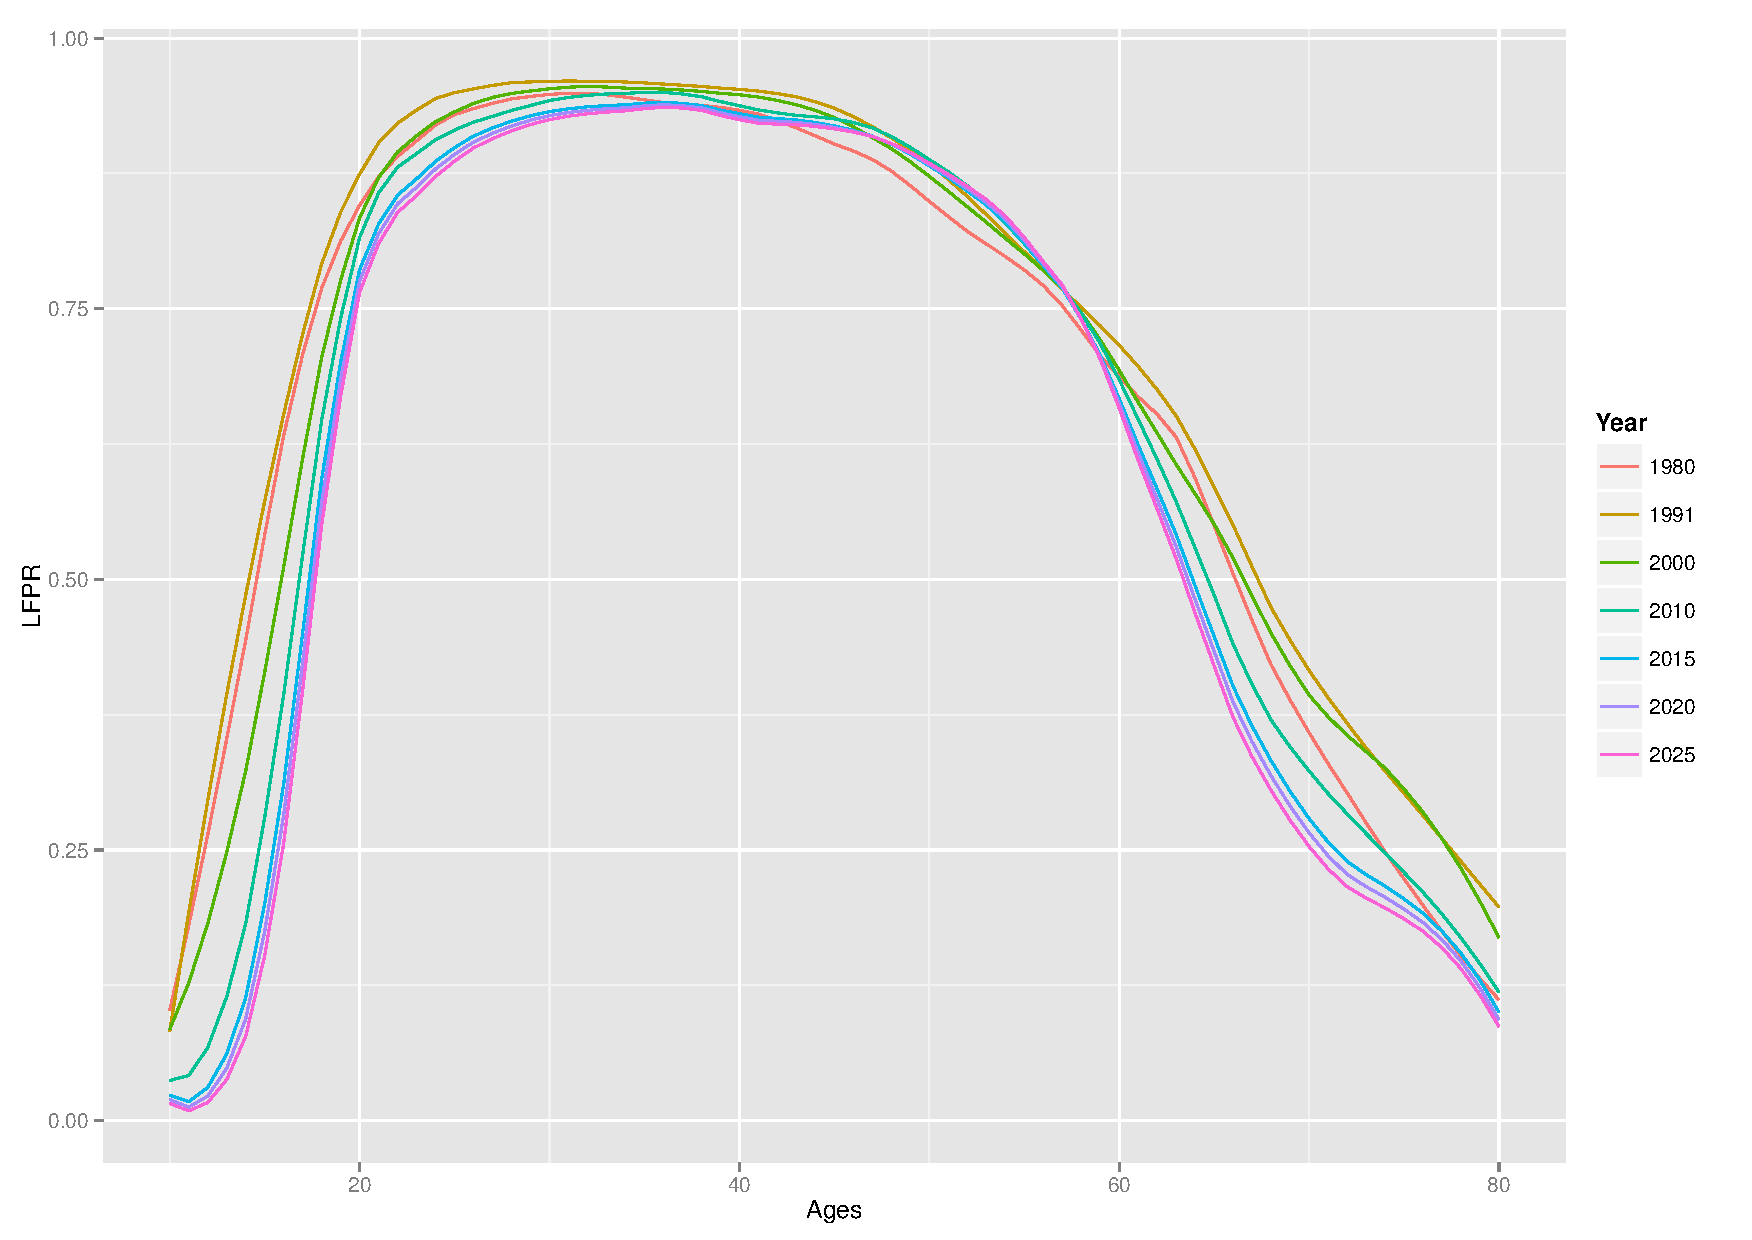
\includegraphics[width=\textwidth]{Graphs/LFPR_select.pdf}
		\end{center}
 		\end{subfigure}
	\legend{Fonte: PNAD}
	\end{figure} \\
	A figura~\ref{fig7.2} mostra as curvas de taxas de atividade para o período entre 1980 e 2025. A taxa de atividade apresenta uma queda nas idades mais jovens e os jovens adultos, que pode ser visto como uma redução do trabalho infantil e do aumento da escolaridade desse segmento \cite{chahad2013mercado}.
	\section{A duração esperada da aposentadoria \label{sec4.3}}
	O processo acelerado de envelhecimento da população brasileira terá um grande impacto na sustentabilidade do RGPS. O aumento na razão de dependência idosa indica que, cada vez mais, uma quantidade crescente de beneficiários dependem de uma quantidade decrescente de contribuintes. Adicionalmente, a queda nas taxas de atividade sinalizam uma mudança no padrão da curva de atividade, marcada pela entrada mais tardia e a saída precoce do mercado de trabalho. \\
	A tabela~\ref{tab2} apresenta os principais resultados desse estudo, a duração esperada da aposentadoria dos homens brasileiros \textit{ELRP}, a expectativa de sobrevida a partir dos 20 anos de idade, $e_{20}$, e a razão $\frac{ELRP}{e_{20}}$, que pode ser interpretada como o percentual da expectativa de vida que será vivida recebendo um benefício de aposentadoria. \\
	\begin{table}[!htb]
	\centering
		\caption{Resultados}
		\label{tab2}
		\begin{tabular}{cccc}
		\toprule
		Ano & ELRP & $e_{20}$ em anos & $\frac{ELRP}{e_{20}}$ \\
		\midrule \midrule
		1980 & 4,925 & 46,54 & 10,58                                    
		\\
		1991 & 5,498 & 47,95 & 11,47                                    
		\\
		2000 & 6,497 & 50,07 & 12,98                                   
		 \\
		2010 & 8,185 & 52,00 & 15,74                                   
		\\
		2015 & 9,052 & 53,02 & 17,07                                    
		\\
		2020 & 9,792 & 54,12 & 18,09                                    
		\\
		2025 & 10,570 & 55,26 & 19,13                                    
		\\ \bottomrule
		\end{tabular}
	\fonte{PNAD e LAHMD}	
	\end{table} \\
	Os resultados sugerem que a duração esperada da aposentadoria aumente aproximadamente 114,40\%, passando de 4,925 anos em 1980 para 10,570 anos em 2025. Esse aumento pode ser atribuído ao aumento da expectativa de vida, apresentado na tabela, e a queda das taxas de atividade. As estimativas aqui apresentadas são uma subestimação das mudanças na duração da aposentadoria, uma vez que elas foram obtidas utilizando dados de período. \\
	\section{Discussão \label{sec4.4}}
	A tabela~\ref{tab3} mostra as estimativas de período (1) e coorte (2), da ELRP, $e_{20}$ e $\tfrac{ELRP}{e_{20}}$ estimadas por \citeonline{lee2001expected}. Os resultados são bastante semelhantes aos encontrados nesse estudo. Observa-se que a ELRP aumentou mais de seis vezes durante o período estudado, e que para a estimativa de coorte, a duração da aposentadoria representava aproximadamente 30\% da sua expectativa de vida após a entrada no mercado de trabalho. \\
	\citeonline{lee2001expected} classifica as estimativas de período e coorte como um intervalo no qual a estimativa de período é o limite inferior, e a estimativa de coorte, o limite superior. O autor supõe dis cenários distintos, no primeiro, um homem de vinte anos avalia a duração da sua aposentadoria com base nos níveis de mortalidade e de taxa de atividade atuais, o que subestima a ELRP real. No segundo cenário, o autor estima que cada coorte consegue prever exatamente o momento da aposentadoria e a sua expectativa de vida, o que superestima a ELRP real. \\
	\\ % pulando linha adicional
	\begin{table}[htb]
	\centering
		\caption{ELRP de homens americanos - Anos Selecionados}
		\label{tab3}
		\begin{tabular}{ccccccc}
		\toprule
		Ano & ELRP$^{(1)}$ & $e_{20}$ em anos$^{(1)}$ & $\frac{ELRP}{e_{20}}$$^{(1)}$ & ELRP$^{(2)}$ & $e_{20}$ em anos$^{(2)}$ & $\frac{ELRP}{e_{20}}$$^{(2)}$\\
		\midrule \midrule
		1850 & 1,68 & 38,41 & 4,4 & 2,65 & 43,70 & 6,1		
		\\		1870 & 0,83 & 41,14 & 2,1 & 3,48 & 44,05 & 7,9 		
		\\		1890 & 2,26 & 40,96 & 5,5 & 4,78 & 46,50 & 10,3 		
		\\		1910 & 3,38 & 41,73 & 7,9 & 6,55 & 49,26 & 13,3 		
		\\		1930 & 4,95 & 44,45 & 10,9 & 9,56 & 53,01 & 18,1 		
		\\		1950 & 6,68 & 46,77 & 13,6 & 13,13 & 55,02 & 23,9 		
		\\		1970 & 8,59 & 49,65 & 17,2 & 14,98 & 56,33 & 26,6 		
		\\		1990 & 12,66 & 52,95 & 23,8 & 16,29 & 57,76 & 28,2 	
		\\ \bottomrule
		\end{tabular}
	\fonte{\cite{lee2001expected}}
	\end{table} \\
	Comparando as tabelas~\ref{tab2} com as estimativas de período da tabela~\ref{tab3} observam-se tendências muito interessantes com relação à ELRP. A duração esperada da aposentadoria de homens americanos nas décadas de 30, 50 e 70 estão muito próximas das estimativas para os anos 1980, 2000 e 2015 respectivamente. Esse resultado fornece evidências que suportam a teoria de que a duração esperada da aposentadoria masculina no Brasil  vai continuar aumentando. Essa diferença de 50 anos observada pode ser explicada pelo fato de que a transição demográfica americana ocorreu entre 1800 e 1940 \cite{greenwood2002us}, enquanto que a brasileira teve início na década de 50 \cite{vasconcelos2012transiccao}. \\
	O Brasil está enfrentando o mesmo problema de nações desenvolvidas. Com o envelhecimento populacional, esses países estão buscando maneiras de aumentar a idade média de aposentadoria e minimizar seu impacto no setor público. Os resultados apresentados aqui indicam que a vida ativa dos homens brasileiros está sendo reduzida, principalmente devido ao aumento do nível de escolarização e da generosidade do RGPS. Esse fenômeno, associado com o aumento da expectativa de vida constitui um cenário perigoso para o RGPS, caracterizado pela saída precoce do mercado de trabalho e altas expectativas de vida.
	%---

    %---
    % Conclusão
    
    \chapter{Conclusão \label{cap5}}
    O objetivo dessa monografia foi estimar a duração esperada da aposentadoria, de acordo com a método proposto por \citeonline{lee2001expected}, para homens no Brasil para o período compreendido entre 1980 e 2025 utilizando dados de mortalidade da Latin America Human Mortality Database e de mercado de trabalho da PNAD. Para o período de projeção, as estimativas de mortalidade e taxa de atividade foram obtidos através da aplicação do modelo Lee--Carter. \\
    O modelo desenvolvido por \citeonline{lee1992modeling} é tradicionalmente utilizado na projeção de taxas de mortalidade. Tendo somente três parâmetros, $a$, $b$ e $k$, as taxas de mortalidade são descritas em função das idades pelos parâmetros $a$ e $b$, e em função do tempo por $k$. A partir desses três parâmetros, as taxas de mortalidade são projetadas. O ajuste do modelo aos dados de mortalidade utilizados foi bastante razoável tendo em vista que a série de dados disponíveis é bastante restrita e que o aumento da mortalidade de jovens adultos ocorrido durante a década de 80 impacta consideravelmente as taxas projetadas para esse grupo etário. \\
    A metodologia utilizada atualmente pelo Ministério da Previdência Social para a projeção das taxas de atividade é extremamente simples, não há projeção. Assume-se a manutanção dos níveis atuais, ou seja não haverá nem aumento ou queda das taxas de atividade. Esse estudo apresentou evidências da queda das taxas de atividade em anos recentes para certos grupos etários, logo, o modelo Lee--Carter foi adaptado para projetá-las. O ajuste do modelo é muito satisfatório, sem distorções graves. A tendência de queda da taxa de atividade é clara, principalmente após a década de 90. \\
    A estimativa da duração da aposentadoria (ELRP) apresenta tendência crescente para todo o período, saindo de um patamar de 4,925 em 1980 para 10,570 em 2025. Quando comparadas com as estimativas encontradas por \citeonline{lee2001expected} para homens americanos, observa-se que os resultandos são consistentes, sustentando a hipótese de que a ELRP deve continuar a crescer. \\
    Uma estimativa mais realista da PEA para fins de medidas relacionadas a previdência não pode incluir pessoas que recebem beneficios previdenciários, então, o próximo passo é rerirá-las do cálculo da ELRP. Além disso, o aumento da mortalidade de jovens aultos prejudica o ajuste do modelo Lee--Carter aos dados de mortalidade, logo, trabalhar com as causas de óbitos permite ajustar a tendência de mortalidade de modo que esse efeito seja minimizado. \\
    A ELRP surge como uma medida que permite avaliar os compromissos do RGPS com seus participantes em função do tempo. É estimada a partir de dados confiáveis através de métodos demográficos e estatísticos com o objetivo de representar de maneira fiel o objeto desse estudo. Além desse objetivo principal, uma nova maneira para projetar a taxa de atividade masculina foi proposta, apresentando resultados plausíveis.
%---
% Bibliografia

\bibliography{abntex2-modelo-references}
%---

\end{document}